%!TEX root=../../main.tex
\begin{chapterpage}{Distributions of random variables}
  \chaptertitle{Distributions of\\[4mm]random variables}
  \label{modeling}
  \chaptersection{randomVariablesSection}
  \chaptersection{binomialModel}
  \chaptersection{normalDist}
  \chaptersection{poisson}
  \chaptersection{distRelatedToBernoulli}
  \chaptersection{correlatedRVs}
  \chaptersection{sectionDistOfRVNotes}
  \chaptersection{sectionDistOfRVExercises}
\end{chapterpage}
\renewcommand{\chapterfolder}{ch_distributions_oi_biostat}

\index{random variable|(}

\chapterintro{{When planning clinical research studies, investigators try to anticipate the results they might see under certain hypotheses. The treatments for some forms of cancer, such as advanced lung cancer, are only effective in a small percentage of patients: typically 20\% or less. Suppose that a study testing a new treatment will be conducted on 20 participants, where the working assumption is that 20\% of the patients will respond to the treatment. How might the possible outcomes of the study be represented, along with their probabilities? It is possible to express various outcomes using the probability notation in the previous chapter, e.g. if $A$ were the event that one patient responds to treatment, but this would quickly become unwieldy. \\

\noindent%
Instead, the anticipated outcome in the study can be represented as a \term{random variable}, which numerically summarizes the possible outcomes of a random experiment. For example, let $X$ represent the number of patients who respond to treatment; a numerical value $x$ can be assigned to each possible outcome, and the probabilities of $1, 2, \dots, x$ patients having a good response can be expressed as $P(X = 1), P(X = 2), \dots , P(X = x)$. The distribution of a random variable specifies the probability of each possible outcome associated with the random variable. \\


\noindent%
This chapter will begin by outlining general properties of random variables and their distributions. The rest of the chapter discusses specific named distributions that are commonly used throughout probability and statistics.}}

%_________________
\section{Random variables}
\label{randomVariablesSection}


\subsection{Distributions of random variables}

Formally, a random variable assigns numerical values to the outcome of a random phenomenon, and is usually written with a capital letter such as $X$, $Y$, or $Z$. 

If a coin is tossed three times, the outcome is the sequence of observed heads and tails. One such outcome might be TTH: tails on the first two tosses, heads on the third. If the random variable $X$ is the number of heads for the three tosses, $X=1$; if $Y$ is the number of tails, then $Y=2$. For the sequence THT, only the order has changed, but the values of $X$ and $Y$ remain the same. For the sequence HHH, however, $X=3$ and $Y=0$. Even in this simple setting, is possible to define other random variables; for example, if $Z$ is the toss when the first H occurs, then $Z=3$ for the first set of tosses (TTH) and 1 for the third set (HHH).  

\begin{figure}[h]
	\centering
	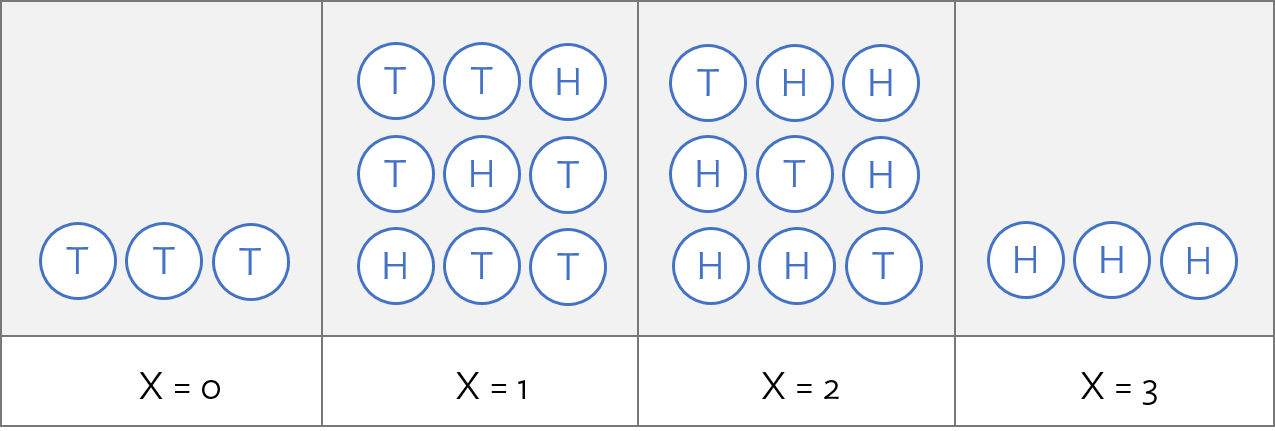
\includegraphics[width=0.70\textwidth]
	{ch_distributions_oi_biostat/figures/coinToss/coinToss.png}
	\caption{Possible outcomes for number of heads in three tosses of a coin.}
	\label{coinToss}
\end{figure}

If probabilities can be assigned to the outcomes in a random phenomenon or study, then those can be used to assign probabilities to values of a random variable.  Using independence, $P(\text{HHH}) = (1/2)^3 = 1/8$.  Since $X$ in the above example can only be three if the three tosses are all heads, $P(X=3) = 1/8$.  The distribution of a random variable is the collection of probabilities for all of the variable's unique values. Figure~\ref{coinToss} shows the eight possible outcomes when a coin is cossed three times: TTT, HTT, THT, TTH, HHT, HTH, THH, HHH. For the first set of tosses, $X = 0$; for the next three, $X=1$, then $X=2$ for the following three tosses and $X=3$ for the last set (HHH).  

Using independence again, each of the 8 outcomes have probability 1/8, so $P(X = 0) = P(X = 3) = 1/8$ and $P(X = 1) = P(X = 2) = 3/8$. Figure~\ref{distCoinTossing} shows the probability distribution for $X$.  Probability distributions for random variables follow the rules for probability; for instance, the sum of the probabilities must be 1.00.  The possible outcomes of $X$ are labeled with a corresponding lower case letter $x$ and subscripts.  The values of X are $x_1=0$, $x_2=1$,  $x_3 = 2$, and $x_4 = 3$; these occur with probabilities $1/8$, $3/8$, $3/8$ and $1/8$.

\begin{figure}[h]
	\centering 
	\begin{tabular}{l rrrr l}
		\hline 
		$i$ & 1 & 2 & 3 & 4 & Total\\
		\hline
		$x_i$ & 0 & 1 & 2 & 3 & --\\
		$P(X = x_i)$ & 1/8 & 3/8 & 3/8 & 1/8 & 8/8 = 1.00\\
	\end{tabular}
	\caption{Tabular form for the distribution of the number of heads in three coin tosses.}
	\label{distCoinTossing}
\end{figure}

\textD{\newpage}

\begin{figure}[h]
	\centering
	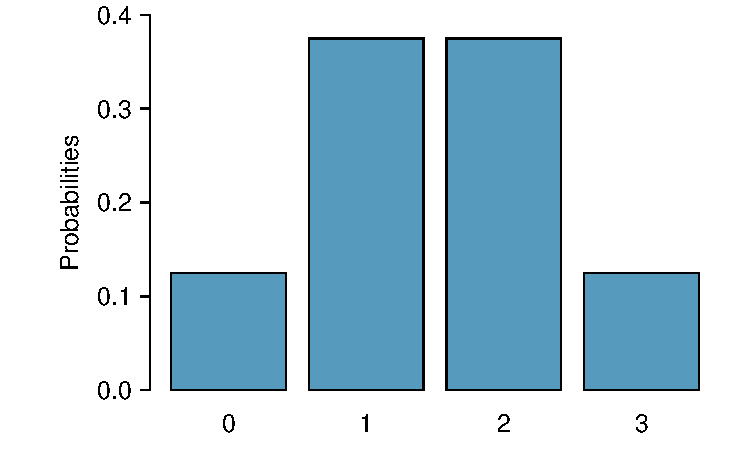
\includegraphics[width=0.56\textwidth]
	{ch_distributions_oi_biostat/figures/barPlotCoinTossing/barPlotCoinTossing.pdf}
	\caption{Bar plot of the distribution of the number of heads in three coin tosses.}
	\label{barPlotCoinTossing}
\end{figure}

Bar graphs can be used to show the distribution of a random variable.  Figure~\ref{barPlotCoinTossing} is a bar graph of the distribution of $X$ in the coin tossing example. When bar graphs are used to show the distribution of a dataset, the heights of the bars show the frequency of observations; in contrast, bar heights for a probability distribution show the probabilities of possible values of a random variable.

$X$ is an example of a \term{discrete random variable} since it takes on a finite number of values.\footnote{Some discrete random variables have an infinite number of possible values, such as all the non-negative integers.} A \term{continuous random variable} can take on any real value in an interval. 

In the hypothetical clinical study described at the beginning of this section, how unlikely would it be for 12 or more patients to respond to the treatment, given that only 20\% of patients are expected to respond? Suppose $X$ is a random variable that will denote the possible number of responding patients, out of a total of 20. $X$ will have the same probability distribution as the number of heads in a 20 tosses of a weighted coin, where the probability of landing heads is 0.20. The graph of the probability distribution for $X$ in Figure~\ref{distRespClinStudy} can be used to approximate this probability. The event of 12 or more consists of nine values (12, 13, \dots, 20); the graph shows that the probabilities for each value is extremely small, so the chance of 12 or more responses must be less than 0.01.\footnote{Formulas in Section~\ref{binomialModel} can be used to show that the exact probability is slightly larger than 0.0001.}

\begin{figure}[h]
	\centering
	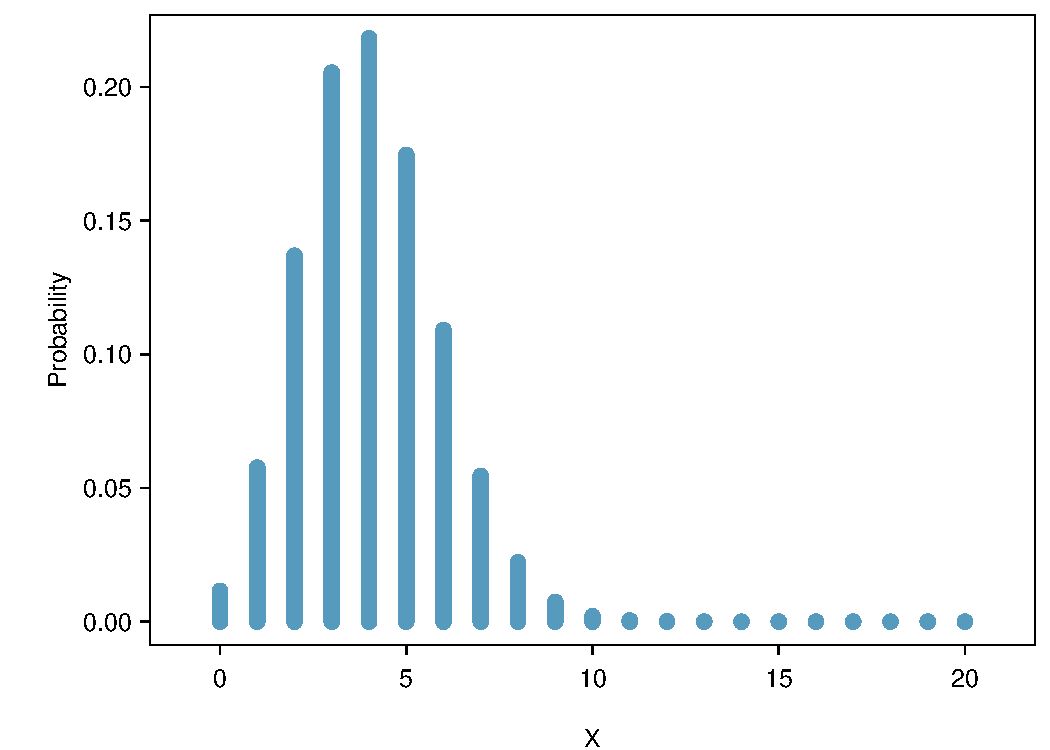
\includegraphics[width=0.72\textwidth]
	{ch_distributions_oi_biostat/figures/distRespClinStudy/distRespClinStudy.pdf}
	\caption{Bar plot of the distribution of the number of responses in a study with 20 participants and response probability 0.20}
	\label{distRespClinStudy}
\end{figure}

\subsection{Expectation} 
\label{section:expectationRandomVariable}

\index{expectation|(}

Just like distributions of data, distributions of random variables also have means, variances, standard deviations, medians, etc.; these characteristics are computed a bit differently for random variables. The mean of a random variable is called its \term{expected value} and written $E(X)$. To calculate the mean of a random variable, multiply each possible value by its corresponding probability and add these products.

\begin{onebox}{Expected value of a discrete random variable}
If $X$ takes on outcomes $x_1$, ..., $x_k$ with probabilities $P(X=x_1)$, ..., $P(X=x_k)$, the expected value of $X$ is the sum of each outcome multiplied by its corresponding probability:
\begin{align}
E(X) 	&= x_1 P(X=x_1) + \cdots + x_k P(X=x_k) \notag \\
&= \sum_{i=1}^{k}x_iP(X=x_i).
\end{align}
The Greek letter $\mu$\index{Greek!mu ($\mu$)} may be used in place of the notation $E(X)$.
\end{onebox}

\begin{examplewrap}
\begin{nexample}{Calculate the expected value of $X$, where $X$ represents the number of heads in three tosses of a fair coin.}
	
	$X$ can take on values 0, 1, 2, and 3. The probability of each $x_k$ is given in Figure~\ref{distCoinTossing}.

\begin{align*}
E(X) &= x_1 P(X = x_1) + \dots + x_k P(X = x_k)\\
&= (0)(P(X=0)) + (1)(P(X=1)) + (2)(P(X=2)) + (3)(P(X = 3)) \\
&= (0)(1/8) + (1)(3/8) + (2)(3/8) + (3)(1/8) = 12/8 \\
&= 1.5.
\end{align*}

The expected value of $X$ is 1.5.
\end{nexample}
\end{examplewrap}

The expected value for a random variable represents the average outcome. For example, $E(X)=1.5$ represents the average number of heads in three tosses of a coin, if the three tosses were repeated many times.\footnote{The expected value $E(X)$ can also be expressed as $\mu$, e.g. $\mu=1.5$}  It often happens with discrete random variables that the expected value is not precisely one of the possible outcomes of the variable.

\marginpar[\raggedright\vspace{-47mm}

$\text{E}(X)$\vspace{1mm}\\\footnotesize Expected Value\\of $X$]{\raggedright\vspace{-47mm}
	
	$\text{E}(X)$\vspace{1mm}\\\footnotesize Expected Value \\of $X$}
\vspace{0mm}

\begin{exercisewrap}
\begin{nexercise}
Calculate the expected value of $Y$, where $Y$ represents the number of heads in three tosses of an unfair coin, where the probability of heads is 0.70.\footnotemark{}
\end{nexercise}
\end{exercisewrap}
\footnotetext{First, calculate the probability distribution. $P(Y=0) = (1 - 0.70)^3 = 0.027$ and $P(Y=3) = (0.70)^3 = 0.343.$ Note that there are three ways to obtain 1 head (HTT, THT, TTH), thus, $P(Y=1) = (3)(0.70)(1 - 0.70)^2 = 0.189$. By the same logic, $P(Y = 2) = (3)(0.70)^2( 1- 0.70) = 0.441$. Thus, $E(Y) = (0)(0.027) + (1)(0.189) + (2)(0.441) + (3)(0.343) = 2.1$. The expected value of $Y$ is 2.1.}

\index{expectation|)}


\textD{\newpage}


\subsection{Variability of random variables} 
\label{section:varianceRandomVariable}

The variability of a random variable can be described with \indexthis{variance}{variance} and \indexthis{standard deviation}{standard deviation}. For data, the variance is computed by squaring deviations from the mean ($x_i - \mu$) and then averaging over the number of values in the dataset (Section~\ref{measuresOfSpread}). 

In the case of a random variable, the squared deviations from the mean of the random variable are used instead, and their sum is weighted by the corresponding probabilities. This weighted sum of squared deviations equals the variance; the standard deviation is the square root of the variance.

\begin{onebox}{Variance of a discrete random variable}
If $X$ takes on outcomes $x_1$, ..., $x_k$ with probabilities $P(X=x_1)$, \dots, $P(X=x_k)$ and expected value $\mu=E(X)$, then the variance of $X$, denoted by $\text{Var}(X)$ or $\sigma^2$, is
\begin{align}
Var(X) &= (x_1-\mu)^2 P(X=x_1) + \cdots \notag + (x_k-\mu)^2 P(X=x_k) \notag \\
&= \sum_{i=1}^{k} (x_i - \mu)^2 P(X=x_i).
\end{align}
The standard deviation of $X$, labeled $SD(X)$ or $\sigma$\index{Greek!sigma ($\sigma$)}, is the square root of the variance.
\end{onebox}%
\marginpar[\raggedright\vspace{-47mm}

$\text{Var}(X)$\vspace{1mm}\\\footnotesize Variance\\of $X$]{\raggedright\vspace{-47mm}
	
	$\text{Var}(X)$\vspace{1mm}\\\footnotesize Variance\\of $X$}

The variance of a random variable can be interpreted as the expectation of the terms $(x_i - \mu)^2$; i.e., $\sigma^2 = E(X - \mu)^2$. While this compact form is not useful for direct computation, it can be helpful for understanding the concept of variability in the context of a random variable; variance is simply the average of the deviations from the mean.


\begin{examplewrap}
\begin{nexample}{Compute the variance and standard deviation of $X$, the number of heads in three tosses of a fair~coin.}
	
	In the formula for the variance, $k = 4$ and $\mu_X = E(X) = 1.5$. 
	\begin{align*}
	\sigma_X^2 &= (x_1-\mu_X)^2P(X=x_1) + \cdots \notag + (x_4-\mu)^2 P(X=x_4) \notag \\
	&= (0- 1.5)^2(1/8) + (1 - 1.5)^2 (3/8) + 
	(2 -1.5)^2 (3/8) + (3-1.5)^2 (1/8) \notag \\
	&= 3/4.
	\end{align*}
	
	The variance is $3/4 = 0.75$ and the standard deviation is $\sqrt{3/4} = 0.866$.  
\end{nexample}
\end{examplewrap}

The coin tossing scenario provides a simple illustration of the mean and variance of a random variable. For the rest of this section, a more realistic example will be discussed\textemdash calculating expected health care costs.

% \label{healthCareCostsEmployee}
In most typical health insurance plans in the United States, members of the plan pay annually in three categories: a monthly premium, a deductible amount that members pay each year before the insurance covers service, and ``out-of-pocket'' costs which include co-payments for each physician visit or prescription.\footnote{The deductible also includes care and supplies that are not covered by insurance.} Picking a new health plan involves estimating costs for the next year based on a person's best guess at the type and number of services that will be needed.

\textD{\newpage}

In 2015, Harvard University offered several alternative plans to its employees. In the Health Maintenance Organization (HMO) plan for employees earning less than \$70,000 per year, the monthly premium was \$79, and the co-payment for each office visit or physical therapy session was \$20. After a new employee examined her health records for the last 10 years, she noticed that in three of the 10 years, she visited the office of her primary care physician only once, for one annual physical. In four of the 10 years, she visited her physician three times: once for a physical, and twice for cases of the flu. In two of the years, she had four visits. In one of the 10 years, she experienced a knee injury that required 3 office visits and 5 physical therapy sessions.

\begin{examplewrap}
\begin{nexample}{Ignoring the cost of prescription drugs, over-the-counter medications, and the annual deductible amount, calculate the expectation and the standard deviation of the expected annual health care cost for this employee.}  \label{example:healthCareCosts}
	
	Let the random variable $X$ denote annual health care costs, where $x_i$ represents the costs in a year for $i$ number of visits. If the last ten years are an accurate picture of annual costs for this employee, $X$ will have four possible values. 
	
	The total cost of the monthly premiums in a single year is $12 \times \$79 = \$948$. The cost of each visit is \$20, so the total visit cost for a year is \$20 times the number of visits. 
	
	For example, the first column in the table contains information about the years in which the employee had one office visit. Adding the \$948 for the annual premium and \$20 for one visit results in $x_{1}=\$968$; $P(X=x_{i}) = 3/10 = 0.30$.
	
	\begin{center}
		\begin{tabular}{l rrrr r}
			\hline
			$i$ & 1 & 2 & 3 & 4 & Sum \\
			\hline
			Number of visits & 1 & 3 & 4 & 8 &\\
			$x_i$ & 968 & 1008 & 1028 & 1108 &  \\
			$P(X=x_i)$ & 0.30 & 0.40 & 0.20 & 0.10 & 1.00 \\
			$x_i P(X=x_i)$ & 290.40 & 403.20 & 205.60 & 110.80 & 1010.00 \\
			\hline
		\end{tabular}
	\end{center}
	The expected cost of health care for a year, $\sum_i x_i P(X = x_i)$, is $\mu=\$1010.00$.
	\begin{center}
		\begin{tabular}{l rrrr r}
			\hline
			$i$ & 1 & 2 & 3 & 4 & Sum \\
			\hline
			Number of visits & 1 & 3 & 4 & 8 &\\
			$x_i$ & 968 & 1008 & 1028 & 1108 &  \\
			$P(X=x_i)$ & 0.30 & 0.40 & 0.20 & 0.10 & 1.00 \\
			$(x_i)P(X=x_i)$ & 290.40 & 403.20 & 205.60 & 110.80 & 1010.00 \\
			\hline
			$x_i - \mu$ & -42.00  & -2.00  & 18.00  & 98.00 & \\
			$(x_i - \mu)^2$ &  1764.00 & 4.00  & 324.00  & 9604 & \\
			$(x_i - \mu)^2 P(X=x_i)$ & 529.20  & 1.60  & 64.80  & 960.40 & 1556.00\\
			\hline
		\end{tabular}
	\end{center}
	The variance of $X$, $\sum_i (x_i - \mu)^2 P(X = x_i)$,  is $\sigma^2 = 1556.00$, and the standard deviation is $\sigma = \$39.45$.\footnotemark{}
\end{nexample}
\end{examplewrap}
\footnotetext{Note that the standard deviation always has the same units as the original measurements.}


\textD{\newpage}


\subsection{Linear combinations of random variables}

Sums of random variables arise naturally in many problems. In the health insurance example, the amount spent by the employee during her next five years of employment can be represented as $X_1 + X_2 + X_3 + X_4 + X_5$, where $X_1$ is the cost of the first year, $X_2$ the second year, etc. If the employee's domestic partner has health insurance with another employer, the total annual cost to the couple would be the sum of the costs for the employee ($X$) and for her partner ($Y$), or $X + Y$. In~each of these examples, it is intuitively clear that the average cost would be the sum of the average of each~term.

Sums of random variables represent a special case of linear combinations of variables.  

\begin{onebox}{Linear combinations of random variables and their expected values}
If $X$ and $Y$ are random variables, then a linear combination of the random variables is given by
\[aX + bY,\] \label{linComboOfRandomVariablesXAndY}
where $a$ and $b$ are constants.  The mean of a linear combination of random variables is 
\[E(aX + bY) = aE(X) + bE(Y) = a\mu_X + b\mu_Y.\]
\end{onebox}

The formula easily generalizes to a sum of any number of random variables. For example, the average health care cost for 5 years, given that the cost for services remains the same, is
\[E(X_1 + X_2 + X_3 + X_4 + X_5) = E(5 X_1) = 5E(X_1) =(5)(1010) = \$5,050.\]

The formula implies that for a random variable $Z$, $E(a + Z) = a + E(Z)$.  This could have been used when calculating the average health costs for the employee by defining $a$ as the fixed cost of the premium ($a=\$948$) and $Z$ as the cost of the physician visits. Thus, the total annual cost for a year could be calculated as: $E(a + Z) = a + E(Z) = \$948 + E(Z) = \$948 + .30(1 \times \$20) + .40(3 \times \$20) + .20(4 \times \$20) + 0.10(8 \times \$20)= \$1,010.00$. 

\begin{exercisewrap}
\begin{nexercise}\label{healthCareCostsPartner}%
Suppose the employee will begin a domestic partnership in the next year. Although she and her companion will begin living together and sharing expenses, they will each keep their existing health insurance plans; both, in fact, have the same plan from the same employer. In the last five years, her partner visited a physician only once in four of the ten years, and twice in the other six years. Calculate the expected total cost of health insurance to the couple in the next year.\footnotemark{}
\end{nexercise}
\end{exercisewrap}
\footnotetext{Let $X$ represent the costs for the employee and $Y$ represent the costs for her partner. $E(X) = \$1,010.00$, as previously calculated. $E(Y) = 948 + 0.4(1 \times \$20) + 0.6(2 \times \$20) = \$980.00$. Thus, $E(X + Y) = E(X) + E(Y) = \$1,010.00 + \$980.00 = \$1,990.00$.}

Calculating the variance and standard deviation of a linear combination of random variables requires more care.  The formula given here requires that the random variables in the linear combination be independent, such that an observation on one of the variables provides no information about the value of the other variable. 

\textD{\newpage}

\begin{onebox}{Variability of linear combinations of random variables}
\[\text{Var}(aX + bY) = a^2 \text{Var}(X) + b^2\text{Var}(Y).\]
This equation is valid only if the random variables are independent of each other.
\end{onebox}

For the transformation $a + bZ$, the variance is $b^{2} \text{Var}(Z)$, since a constant $a$ has variance 0.  When $b = 1$, variance of $a + Z$ is $\text{Var}(Z)$\textemdash adding a constant to a random variable has no effect on the variability of the random variable.

\begin{examplewrap}
\begin{nexample}{Calculate the variance and standard deviation for the combined cost of next year's health care for the two partners, assuming that the costs for each person are independent.}\label{sdHealthCostsPartners} 

Let $X$ represent the sum of costs for the employee and $Y$ the sum of costs for her partner.
	
First, calculate the variance of health care costs for the partner. The partner's costs are the sum of the annual fixed cost and the variable annual costs, so the variance will simply be the variance of the variable costs. If $Z$ represents the component of the variable costs, $E(Z) = 0.4(1 \times \$20) + 0.6(2 \times \$20) = \$8 + \$24 = \$32$. Thus, the variance of $Z$ equals
\[\textrm{Var}(Z) = 0.4(20 - 32)^2 + 0.6(40 - 32)^2 = 96. \]

Under the assumption of independence, Var$(X + Y)$ = $\text{Var}(X) + \text{Var}(Y) = 1556 + 96 = 1652$, and the standard deviation is $\sqrt{1652} = \$40.64$.
\end{nexample}
\end{examplewrap}

The example of health insurance costs has been simplified to make the calculations clearer.  It ignores the fact that many plans have a deductible amount, and that plan members pay for services at different rates before and after the deductible has been reached. Often, insured individuals no longer need to pay for services at all once a maximum amount has been reached in a year. The example also assumes that the proportions of number of physician visits per year, estimated from the last 10 years, can be treated as probabilities measured without error. Had a different timespan been chosen, the proportions might well have been different.  

It also relies on the assumption that health care costs for the two partners are independent.  Two individuals living together may pass on infectious diseases like the flu, or may participate together in activities that lead to similar injuries, such as skiing or long distance running.  Section~\ref{correlatedRVs} shows how to adjust a variance calculation when independence is unrealistic.


\index{random variable|)}


%__________
\section{Binomial distribution}
\label{binomialModel}

The hypothetical clinical study and coin tossing example discussed earlier in this chapter are both examples of experiments that can be modeled with a binomial distribution. The binomial distribution is a more general case of another named distribution, the Bernoulli distribution.

\index{distribution!binomial|(}

\subsection{Bernoulli distribution}
\label{bernoulli}

\index{distribution!Bernoulli|(}

Psychologist Stanley Milgram\index{Milgram, Stanley} began a series of experiments in 1963 to study the effect of authority on obedience. In a typical experiment, a participant would be ordered by an authority figure to give a series of increasingly severe shocks to a stranger. Milgram found that only about 35\% of people would resist the authority and stop giving shocks before the maximum voltage was reached. Over the years, additional research suggested this number is approximately consistent across communities and time.\footnote{Find further information on Milgram's experiment at \par \ \ \hspace{0.2mm}\ \oiRedirect{textbook-milgram}{www.cnr.berkeley.edu/ucce50/ag-labor/7article/article35.htm}.}

Each person in Milgram's experiment can be thought of as a \term{trial}. Suppose that a trial is labeled a \term{success} if the person refuses to administer the worst shock. If the person does administer the worst shock, the trial is a \term{failure}. The \term{probability of a success} can be written as $p=0.35$. The probability of a failure is sometimes denoted with $q=1-p$.

When an individual trial only has two possible outcomes, it is called a \termsub{Bernoulli random variable}{distribution!Bernoulli}. It is arbitrary as to which outcome is labeled success. 

Bernoulli random variables are often denoted as \resp{1} for a success and \resp{0} for a failure. Suppose that ten trials are observed, of which 6 are successes and 4 are failures:
\begin{center}
	\resp{0} \resp{1} \resp{1} \resp{1} \resp{1} \resp{0} \resp{1} \resp{1} \resp{0} \resp{0}.
\end{center}
The \term{sample proportion}, $\hat{p}$, is the sample mean of these observations:
\begin{eqnarray*}
	\hat{p} = \frac{\text{\# of successes}}{\text{\# of trials}} = \frac{0+1+1+1+1+0+1+1+0+0}{10} = 0.6.
\end{eqnarray*}%
Since \resp{0} and \resp{1} are numerical outcomes, the {mean} and {standard deviation} of a Bernoulli random variable can be defined. If ${p}$ is the true probability of a success, then the mean of a Bernoulli random variable $X$ is given by
\begin{align*}
\mu = E[X] &= P(X=0)\times0 + P(X=1)\times1 \\
&= (1-p)\times0 + p\times 1 = 0+p = p.
\end{align*}
Similarly, the variance of $X$ can be computed:
\begin{align*}
\sigma^2 &= {P(X=0)(0-p)^2 + P(X=1)(1-p)^2} \\
&= {(1-p)p^2 + p(1-p)^2} = {p(1-p).}
\end{align*}
The standard deviation is $\sigma=\sqrt{p(1-p)}$.

\textD{\newpage}

\begin{onebox}{Bernoulli random variable}
If $X$ is a random variable that takes value 1 with probability of success $p$ and 0 with probability $1-p$, then $X$ is a Bernoulli random variable with mean $p$ and standard deviation $\sqrt{p(1-p)}$.
\end{onebox}

Suppose $X$ represents the outcome of a single toss of a fair coin, where heads is labeled success. $X$ is a Bernoulli random variable with probability of success $p = 0.50$; this can be expressed as $X \sim \textrm{Bern}(p)$, or specifically, $X \sim \textrm{Bern}(0.50)$. It is essential to specify the probability of success when characterizing a Bernoulli random variable. For example, although the outcome of a single toss of an unfair coin can also be represented by a Bernoulli, it will have a different probability distribution since $p$ does not equal 0.50 for an unfair coin. 

The success probability $p$ is the \term{parameter} of the distribution, and identifies a specific Bernoulli distribution out of the entire family of Bernoulli distributions where $p$ can be any value between 0 and 1 (inclusive). \marginpar[\raggedright\vspace{-12mm}

$\textrm{Bern}(p)$\vspace{1mm}\\\footnotesize Bernoulli dist.\\with $p$ prob. of success]{\raggedright\vspace{-12mm}
	
	$\textrm{Bern}(p)$\vspace{1mm}\\\footnotesize Bernoulli dist.\\with $p$ prob. of success} 

\index{distribution!Bernoulli|)}

\begin{examplewrap}
\begin{nexample}{Suppose that four individuals are randomly selected to participate in Milgram's experiment. What is the chance that there will be exactly one successful trial, assuming independence between trials? Suppose that the probability of success remains 0.35.}\label{oneRefuser}
	
	Consider a scenario in which there is one success (i.e., one person refuses to give the strongest shock). Label the individuals as $A$, $B$, $C$, and $D$:
	
	\begin{align*}
	&P(A=\text{\resp{refuse}},\text{ }B=\text{\resp{shock}},\text{ }C=\text{\resp{shock}},\text{ }D=\text{\resp{shock}}) \\
	&\quad =  P(A=\text{\resp{refuse}})\ P(B=\text{\resp{shock}})\ P(C=\text{\resp{shock}})\ P(D=\text{\resp{shock}}) \\
	&\quad =  (0.35)  (0.65)  (0.65)  (0.65) = (0.35)^1 (0.65)^3 = 0.096.
	\end{align*}
	
	However, there are three other possible scenarios: either $B$, $C$, or $D$ could have been the one to refuse. In each of these cases, the probability is also $(0.35)^1(0.65)^3$. These four scenarios exhaust all the possible ways that exactly one of these four people could refuse to administer the most severe shock, so the total probability of one success is $(4)(0.35)^1(0.65)^3 = 0.38$.
\end{nexample}
\end{examplewrap}


\textD{\newpage}


\subsection{The binomial distribution}

The Bernoulli distribution is unrealistic in all but the simplest of settings. However, it is a useful building block for other distributions. The \termsub{binomial distribution}{distribution!binomial} describes the probability of having exactly $k$ successes in $n$ independent Bernoulli trials with probability of a success $p$. In Example~\ref{oneRefuser}, the goal was to calculate the probability of 1 success out of 4 trials, with probability of success 0.35 ($n=4$, $k=1$, $p=0.35$). 

Like the Bernoulli distribution, the binomial is a discrete distribution, and can take on only a finite number of values. A binomial variable has values 0, 1, 2, \dots, $n$.

A general formula for the binomial distribution can be developed from re-examining Example~\ref{oneRefuser}. There were four individuals who could have been the one to refuse, and each of these four scenarios had the same probability. Thus, the final probability can be written as:
\begin{eqnarray}
[\text{\# of scenarios}] \times P(\text{single scenario}.)
\label{genBinomialFormula}
\end{eqnarray}
The first component of this equation is the number of ways to arrange the $k=1$ successes among the $n=4$ trials. The second component is the probability of any of the four (equally probable) scenarios.

Consider $P($single scenario$)$ under the general case of $k$ successes and $n-k$ failures in the $n$ trials. In any such scenario, the Multiplication Rule for independent events can be applied:
\begin{eqnarray*}
	p^k(1-p)^{n-k}.
\end{eqnarray*}

Secondly, there is a general formula for the number of ways to choose $k$ successes in $n$ trials, i.e. arrange $k$ successes and $n-k$ failures:
\begin{eqnarray*}
	{n\choose k} = \frac{n!}{k!(n-k)!}.
\end{eqnarray*}
The quantity ${n\choose k}$ is read \term{n choose k}.\footnote{Other notation for $n$ choose $k$ includes $_nC_k$, $C_n^k$, and $C(n,k)$.} The exclamation point notation (e.g. $k!$) denotes a \term{factorial}\label{factorialDefinitionInTheBinomialSection} expression.\footnote{$0! = 1$ \label{zeroFactorial}, $1! = 1$, $2! = 2 \times 1 = 2$, $\dots$, $n! = n\times (n-1) \times \dots 2 \times 1$.}

Using the formula, the number of ways to choose $k=1$ successes in $n=4$ trials can be computed as:
\begin{eqnarray*}
	{4 \choose 1} = \frac{4!}{1!(4-1)!} =  \frac{4!}{1!3!} 
	= \frac{4\times3\times2\times1}{(1)(3\times2\times1)} = 4.
\end{eqnarray*}

Substituting $n$ choose $k$ for the number of scenarios and $p^k(1-p)^{n-k}$ for the single scenario probability in Equation~(\ref{genBinomialFormula}) yields the general binomial formula. 

\textD{\newpage}

\begin{onebox}{Binomial distribution}
Suppose the probability of a single trial being a success is $p$. The probability of observing exactly $k$ successes in $n$ independent trials is given by\vspace{-1mm}
\begin{eqnarray}
P(X = k) = {n\choose k}p^k(1-p)^{n-k} = \frac{n!}{k!(n-k)!}p^k(1-p)^{n-k}.
\label{binomialFormula}
\end{eqnarray}
Additionally, the mean, variance, and standard deviation of the number of observed successes are, respectively\vspace{-2mm}
\begin{align}
\mu &= np
  &\sigma^2 &= np(1-p)
  &\sigma &= \sqrt{np(1-p)}.
\label{binomialStats}
\end{align}
A binomial random variable $X$ can be expressed as $X \sim \textrm{Bin}(n, p)$.
\end{onebox}%
\marginpar[\raggedright\vspace{-45mm}

$\textrm{Bin}(n, p)$\vspace{1mm}\\\footnotesize Binomial dist.\\with $n$ trials\\\& $p$ prob. of success]{\raggedright\vspace{-45mm}
	
	$\textrm{Bin}(n, p)$\vspace{1mm}\\\footnotesize Binomial dist.\\with $n$ trials\\\& $p$ prob. of success} 

\begin{onebox}{Is it binomial? Four conditions to check.}
\label{isItBinomialTipBox}%
(1) The trials are independent. \\
(2) The number of trials, $n$, is fixed. \\
(3) Each trial outcome can be classified as a \emph{success} or \emph{failure}. \\
(4) The probability of a success, $p$, is the same for each trial.
\end{onebox}

\begin{examplewrap}
\begin{nexample}{What is the probability that 3 of 8 randomly selected participants will refuse to administer the worst shock?}
	
	First, check the conditions for applying the binomial model. The number of trials is fixed ($n=8$) and each trial outcome can be classified as either success or failure. The sample is random, so the trials are independent, and the probability of success is the same for each trial. 
	
	For the outcome of interest, $k=3$ successes occur in $n=8$ trials, and the probability of a success is $p=0.35$. Thus, the probability that 3 of 8 will refuse is given by
	\begin{eqnarray*}
		P(X =3) = { 8 \choose 3}(0.35)^3(1-0.35)^{8-3}
		&=& \frac{8!}{3!(8-3)!}(0.35)^3(1-0.35)^{8-3} \\
		&=& (56)(0.35)^3(0.65)^5 \\
		&=& 0.28.
	\end{eqnarray*}
\end{nexample}
\end{examplewrap}

\begin{examplewrap}
\begin{nexample}{What is the probability that at most 3 of 8 randomly selected participants will refuse to administer the worst shock?}
	
	The event of at most 3 out of 8 successes can be thought of as the combined probability of 0, 1, 2, and 3 successes. Thus, the probability that at most 3 of 8 will refuse is given by:
	\begin{align*}
	P(X \leq 3) &= P(X = 0) + P(X = 1) + P(X = 2) + P(X = 3) \\
	&= { 8 \choose 0}(0.35)^0(1-0.35)^{8-0} + { 8 \choose 1}(0.35)^1(1-0.35)^{8-1} \\
	& \qquad + { 8 \choose 2}(0.35)^2(1-0.35)^{8-2} + { 8 \choose 3}(0.35)^3(1-0.35)^{8-3} \\
	&= (1)(0.35)^0(1-0.35)^{8} + (8)(0.35)^1(1-0.35)^{7} \\
	& \qquad + (28)(0.35)^2(1-0.35)^{6} + (56)(0.35)^3(1-0.35)^{5}\\
	&= 0.706.
	\end{align*}
\end{nexample}
\end{examplewrap}

\begin{examplewrap}
\begin{nexample}{If 40 individuals were randomly selected to participate in the experiment, how many individuals would be expected to refuse to administer the worst shock? What is the standard deviation of the number of people expected to refuse?}
	
	Both quantities can directly be computed from the formulas in Equation~(\ref{binomialStats}). The expected value (mean) is given by: $\mu=np = 40\times 0.35 = 14$. The standard deviation is: $\sigma = \sqrt{np(1-p)} = \sqrt{40\times 0.35\times 0.65} = 3.02$.
\end{nexample}
\end{examplewrap}

\begin{exercisewrap}
\begin{nexercise}
The probability that a smoker will develop a severe lung condition in their lifetime is about 0.30. Suppose that 5 smokers are randomly selected from the population. What is the probability that (a) one will develop a severe lung condition? (b) that no more than one will develop a severe lung condition? (c) that at least one will develop a severe lung condition?\footnotemark{}
\end{nexercise}
\end{exercisewrap}
\footnotetext{Let $p = 0.30$; $X \sim \textrm{Bin}(5, 0.30)$. (a) $P(X=1) = {5 \choose 1}(0.30)^1(1-0.30)^{5-1} = 0.36$ (b) $P(X \leq 1) = P(X=0) + P(X=1) = {5 \choose 0}(0.30)^0(1-0.30)^{5-0} + 0.36 = 0.53$ (c) $P(X \geq 1) = 1 - P(X=0) = 1 - 0.36 = 0.83$}

\index{distribution!binomial|)}


%_________________
\section{Normal distribution}
\label{normalDist}

\index{distribution!normal|(}

Among the many distributions seen in practice, one is by far the most common: the \termsub{normal distribution}{distribution!normal}, which has the shape of a symmetric, unimodal bell curve. Many variables are nearly normal, which makes the normal distribution useful for a variety of problems. For example, characteristics such as human height closely follow the normal distribution.


\subsection{Normal distribution model}

The normal distribution model always describes a symmetric, unimodal, bell-shaped curve. However, the curves can differ in center and spread; the model can be adjusted using mean and standard deviation. Changing the mean shifts the bell curve to the left or the right, while changing the standard deviation stretches or constricts the curve. Figure~\ref{twoSampleNormals} shows the normal distribution with mean $0$ and standard deviation $1$ in the left panel and the normal distribution with mean $19$ and standard deviation $4$ in the right panel. Figure~\ref{twoSampleNormalsStacked} shows these distributions on the same axis.

\begin{figure}[hht]
\centering
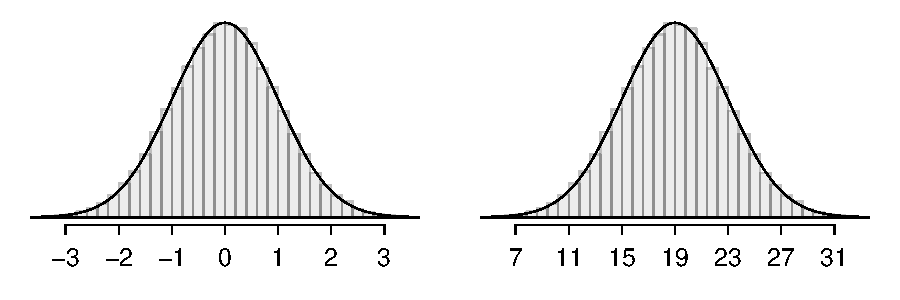
\includegraphics[width=0.85\textwidth]{ch_distributions_oi_biostat/figures/twoSampleNormals/twoSampleNormals}
\caption{Both curves represent the normal distribution; however, they differ in their center and spread. The normal distribution with mean 0 and standard deviation 1 is called the \term{standard normal distribution}.}
\label{twoSampleNormals}
\end{figure}

\begin{figure}[hht]
\centering
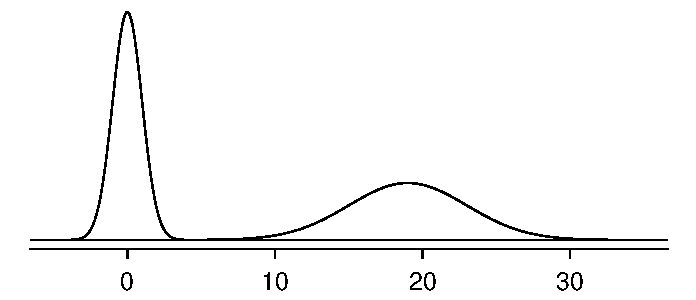
\includegraphics[width=0.6\textwidth]{ch_distributions_oi_biostat/figures/twoSampleNormalsStacked/twoSampleNormalsStacked}
\caption{The normal models shown in Figure~\ref{twoSampleNormals} but plotted together and on the same scale.}
\label{twoSampleNormalsStacked}
\end{figure}

For any given normal distribution with mean $\mu$ and standard deviation $\sigma$, the distribution can be written as $N(\mu, \sigma)$; $\mu$ and $\sigma$ are the parameters of the normal distribution. \marginpar[\raggedright\vspace{-5mm}

$N(\mu, \sigma)$\vspace{1mm}\\\footnotesize Normal dist.\\with mean $\mu$\\\& st. dev. $\sigma$]{\raggedright\vspace{-5mm}

$N(\mu, \sigma)$\vspace{1mm}\\\footnotesize Normal dist.\\with mean $\mu$\\\& st. dev. $\sigma$} For example, $N(0, 1)$ refers to the standard normal distribution, as shown in Figure~\ref{twoSampleNormals}. 

Unlike the Bernoulli and binomial distributions, the normal distribution is a continuous distribution. 


\textD{\newpage}


\subsection{Standardizing with Z-scores}

The \term{Z-score}\marginpar[\raggedright\vspace{-3mm}

$Z$\vspace{1mm}\\\footnotesize Z-score, the\\standardized\\observation]{\raggedright\vspace{-3mm}
	
	$Z$\vspace{1mm}\\\footnotesize Z-score, the\\standardized\\observation}\index{Z@$Z$} of an observation quantifies how far the observation is from the mean, in units of standard deviation(s). If $x$ is an observation from a distribution $N(\mu, \sigma)$, the Z-score is mathematically defined as:
\begin{align*}
	Z = \frac{x-\mu}{\sigma}.
\end{align*}

An observation equal to the mean has a Z-score of 0. Observations above the mean have positive Z-scores, while observations below the mean have negative Z-scores. For example, if an observation is one standard deviation above the mean, it has a Z-score of 1; if it is 1.5 standard deviations below the mean, its Z-score is -1.5. 

Z-scores can be used to identify which observations are more extreme than others, and are especially useful when comparing observations from different normal distributions. One observation $x_1$ is said to be more unusual than another observation $x_2$ if the absolute value of its Z-score is larger than the absolute value of the other observation's Z-score: $|Z_1| > |Z_2|$. In other words, the further an observation is from the mean in either direction, the more extreme it is. 

\begin{examplewrap}
\begin{nexample}{The SAT and the ACT are two standardized tests commonly used for college admissions in the United States. The distribution of test scores are both nearly normal. For the SAT, $N(1500, 300)$; for the ACT, $N(21, 5)$. While some colleges request that students submit scores from both tests, others allow students the choice of either the ACT or the SAT. Suppose that one student scores an 1800 on the SAT (Student A) and another scores a 24 on the ACT (Student B). A college admissions officer would like to compare the scores of the two students to determine which student performed better.}\label{actSAT}
		
Calculate a Z-score for each student; i.e., convert $x$ to Z.
		
Using $\mu_{SAT}=1500$, $\sigma_{SAT}=300$, and $x_{A}=1800$, find Student A's Z-score:
\begin{align*}
	Z_{A} = \frac{x_{A} - \mu_{SAT}}{\sigma_{SAT}} = \frac{1800-1500}{300} = 1.
\end{align*}

For Student B:
\begin{align*}
	Z_{B} = \frac{x_{B} - \mu_{ACT}}{\sigma_{ACT}} = \frac{24 - 21}{5} = 0.6.
\end{align*}

Student A's score is 1 standard deviation above average on the SAT, while Student B's score is 0.6 standard deviations above the mean on the ACT. As illustrated in Figure~\ref{satActNormals}, Student A's score is more extreme, indicating that Student A has scored higher with respect to other scores than Student B.
\end{nexample}
\end{examplewrap}

\begin{figure}[h]
\centering
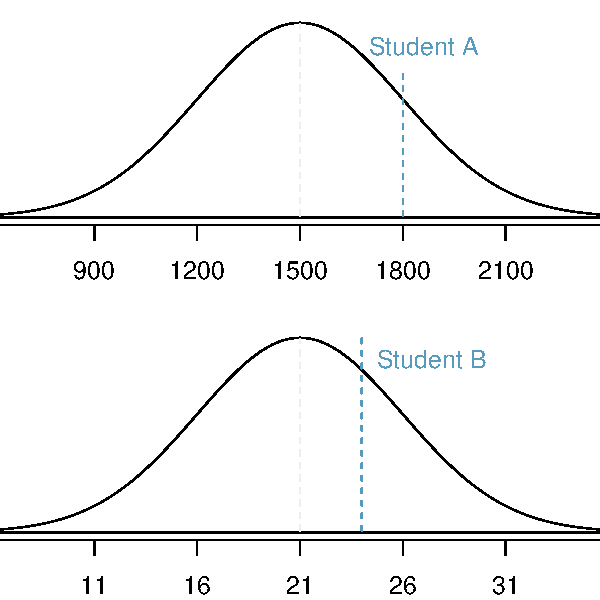
\includegraphics[width=0.5\textwidth]{ch_distributions_oi_biostat/figures/satActNormals/satActNormals}
\caption{Scores of Students A and B plotted on the distributions of SAT and ACT scores.}
\label{satActNormals}
\end{figure}

\begin{onebox}{The Z-score}
The Z-score of an observation quantifies how far the observation is from the mean, in units of standard deviation(s). The Z-score for an observation $x$ that follows a distribution with mean $\mu$ and standard deviation $\sigma$ can be calculated using
\begin{align*}
Z = \frac{x-\mu}{\sigma}.
\end{align*}
\end{onebox}

\textD{\newpage}

\begin{examplewrap}
\begin{nexample}{How high would a student need to score on the ACT to have a score equivalent to Student A's score of 1800 on the SAT?} 

As shown in Example~\ref{satActNormals}, a score of 1800 on the SAT is 1 standard deviation above the mean. ACT scores are normally distributed with mean 21 and standard deviation 5. To convert a value from the standard normal curve (Z) to one on a normal distribution $N(\mu, \sigma)$:

\begin{align*}
x = \mu + Z\sigma.
\end{align*}

Thus, a student would need a score of $21 + 1(5) = 26$ on the ACT to have a score equivalent to 1800 on the SAT. 
\end{nexample}
\end{examplewrap}

\begin{exercisewrap}
\begin{nexercise}\label{nhanes_bp}%
Systolic blood pressure (SBP) for adults in the United States aged 18-39 follow an approximate normal distribution, $N(115, 17.5)$. As age increases, systolic blood pressure also tends to increase. Mean systolic blood pressure for adults 60 years of age and older is 136 mm Hg, with standard deviation 40 mm Hg. Systolic blood pressure of 140 mm Hg or higher is indicative of hypertension (high blood pressure). 
(a) How many standard deviations away from the mean is a 30-year-old with systolic blood pressure of 125 mm Hg? (b) Compare how unusual a systolic blood pressure of 140 mm Hg is for a 65-year-old, versus a 30-year-old.\footnotemark{}
\end{nexercise}
\end{exercisewrap}
\footnotetext{(a) Calculate the $Z$-score: $\frac{\overline{x} - \mu}{\sigma} = \frac{125 - 115}{17.5} = 0.571$. A 30-year-old with systolic blood pressure of 125 mm Hg is about 0.6 standard deviations above the mean. (b) For $x_1=140$ mm Hg: $Z_1 = \frac{x_1 - \mu}{\sigma} = \frac{140 - 115}{17.5} = 1.43$. For $x_2=140$ mm Hg: $Z_2 = \frac{x_2 - \mu}{\sigma} = \frac{140 - 136}{40} = 0.1$. While an SBP of 140 mm Hg is almost 1.5 standard deviations above the mean for a 30-year-old, it is only 0.1 standard deviations above the mean for a 65-year-old.}

% cite nhanes_bp, SD calculated as SE * sqrt(n) from tables


\textD{\newpage}


\subsection{The empirical rule}\label{empiricalRule}

The empirical rule (also known as the 68-95-99.7 rule) states that for a normal distribution, almost all observations will fall within three standard deviations of the mean. Specifically, 68\% of observations are within one standard deviation of the mean, 95\% are within two SD's, and 99.7\% are within three SD's. 

\begin{figure}[h]
	\centering
	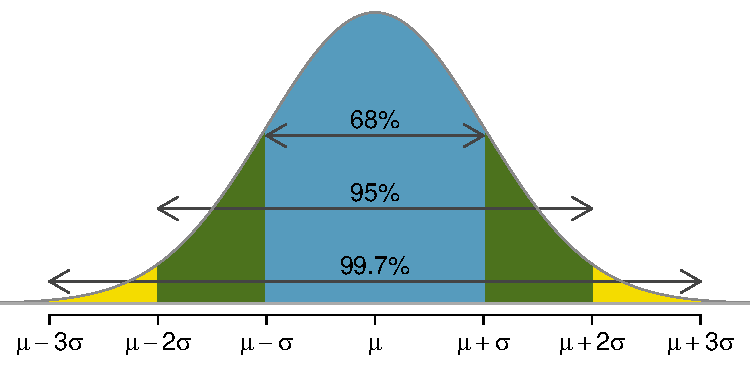
\includegraphics[width=0.7\textwidth]{ch_distributions_oi_biostat/figures/6895997/6895997}
	\caption{Probabilities for falling within 1, 2, and 3 standard deviations of the mean in a normal distribution.}
	\label{6895997}
\end{figure}

While it is possible for a normal random variable to take on values 4, 5, or even more standard deviations from the mean, these occurrences are extremely rare if the data are nearly normal. For example, the probability of being further than 4 standard deviations from the mean is about 1-in-30,000.

\subsection{Calculating normal probabilities}

The normal distribution is a continuous probability distribution. Recall from Section~\ref{introProbDistributions} that the total area under the density curve is always equal to 1, and the probability that a variable has a value within a specified interval is the area under the curve over that interval. By using either statistical software or normal probability tables, the normal model can be used to identify a probability or percentile based on the corresponding Z-score (and vice versa). 

\begin{figure}[h]
	\centering
	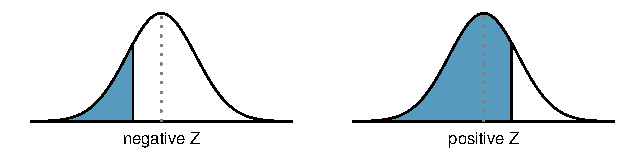
\includegraphics[width=0.95\textwidth]{ch_distributions_oi_biostat/figures/normalTails/normalTails}
	\caption{The area to the left of $Z$ represents the percentile of the observation.}
	\label{normalTails}
\end{figure}

\textD{\newpage}

A \term{normal probability table} is given in Appendix~\vref{normalProbabilityTable} and abbreviated in Figure~\ref{zTableShort}. This table can be used to identify the \term{percentile} corresponding to any particular Z-score; for instance, the percentile of $Z=0.43$ is shown in row $0.4$ and column $0.03$ in Figure~\ref{zTableShort}: 0.6664, or the $66.64^{th}$ percentile. First, find the proper row in the normal probability table up through the first decimal, and then determine the column representing the second decimal value. The intersection of this row and column is the percentile of the observation. This value also represents the probability that the standard normal variable Z takes on a value of 0.43 or less; i.e. $P(Z \leq 0.43) = 0.6664$.

The table can also be used to find the Z-score associated with a percentile. For example, to identify Z for the $80^{th}$ percentile, look for the value closest to 0.8000 in the middle portion of the table: 0.7995. The Z-score for the $80^{th}$ percentile is given by combining the row and column Z values: 0.84.

\begin{figure}
	\centering
	\begin{tabular}{c | rrrrr | rrrrr |}
		\cline{2-11}
		&&&& \multicolumn{4}{c}{Second decimal place of $Z$} &&& \\
		\cline{2-11}
		$Z$ & 0.00 & 0.01 & 0.02 & \highlightT{0.03} & \highlightO{0.04} & 0.05 & 0.06 & 0.07 & 0.08 & 0.09 \\
		\hline
		\hline
		0.0 & \scriptsize{0.5000} & \scriptsize{0.5040} & \scriptsize{0.5080} & \scriptsize{0.5120} & \scriptsize{0.5160} & \scriptsize{0.5199} & \scriptsize{0.5239} & \scriptsize{0.5279} & \scriptsize{0.5319} & \scriptsize{0.5359} \\
		0.1 & \scriptsize{0.5398} & \scriptsize{0.5438} & \scriptsize{0.5478} & \scriptsize{0.5517} & \scriptsize{0.5557} & \scriptsize{0.5596} & \scriptsize{0.5636} & \scriptsize{0.5675} & \scriptsize{0.5714} & \scriptsize{0.5753} \\
		0.2 & \scriptsize{0.5793} & \scriptsize{0.5832} & \scriptsize{0.5871} & \scriptsize{0.5910} & \scriptsize{0.5948} & \scriptsize{0.5987} & \scriptsize{0.6026} & \scriptsize{0.6064} & \scriptsize{0.6103} & \scriptsize{0.6141} \\
		%  May comment out 0.0-0.2 to make extra space. Then insert the following line:
		%  $\vdots$ &   $\vdots$ &   $\vdots$ &   $\vdots$ &   $\vdots$ &   $\vdots$ &   $\vdots$ &   $\vdots$ &   $\vdots$ &   $\vdots$ &   $\vdots$ \\
		0.3 & \scriptsize{0.6179} & \scriptsize{0.6217} & \scriptsize{0.6255} & \scriptsize{0.6293} & \scriptsize{0.6331} & \scriptsize{0.6368} & \scriptsize{0.6406} & \scriptsize{0.6443} & \scriptsize{0.6480} & \scriptsize{0.6517} \\
		\highlightT{0.4} & \scriptsize{0.6554} & \scriptsize{0.6591} & \scriptsize{0.6628} & \highlightT{\scriptsize{0.6664}} & \scriptsize{0.6700} & \scriptsize{0.6736} & \scriptsize{0.6772} & \scriptsize{0.6808} & \scriptsize{0.6844} & \scriptsize{0.6879} \\
		\hline
		0.5 & \scriptsize{0.6915} & \scriptsize{0.6950} & \scriptsize{0.6985} & \scriptsize{0.7019} & \scriptsize{0.7054} & \scriptsize{0.7088} & \scriptsize{0.7123} & \scriptsize{0.7157} & \scriptsize{0.7190} & \scriptsize{0.7224} \\
		0.6 & \scriptsize{0.7257} & \scriptsize{0.7291} & \scriptsize{0.7324} & \scriptsize{0.7357} & \scriptsize{0.7389} & \scriptsize{0.7422} & \scriptsize{0.7454} & \scriptsize{0.7486} & \scriptsize{0.7517} & \scriptsize{0.7549} \\
		0.7 & \scriptsize{0.7580} & \scriptsize{0.7611} & \scriptsize{0.7642} & \scriptsize{0.7673} & \scriptsize{0.7704} & \scriptsize{0.7734} & \scriptsize{0.7764} & \scriptsize{0.7794} & \scriptsize{0.7823} & \scriptsize{0.7852} \\
		\highlightO{0.8} & \scriptsize{0.7881} & \scriptsize{0.7910} & \scriptsize{0.7939} & \scriptsize{0.7967} & \highlightO{\scriptsize{0.7995}} & \scriptsize{0.8023} & \scriptsize{0.8051} & \scriptsize{0.8078} & \scriptsize{0.8106} & \scriptsize{0.8133} \\
		0.9 & \scriptsize{0.8159} & \scriptsize{0.8186} & \scriptsize{0.8212} & \scriptsize{0.8238} & \scriptsize{0.8264} & \scriptsize{0.8289} & \scriptsize{0.8315} & \scriptsize{0.8340} & \scriptsize{0.8365} & \scriptsize{0.8389} \\
		\hline
		\hline
		1.0 & \scriptsize{0.8413} & \scriptsize{0.8438} & \scriptsize{0.8461} & \scriptsize{0.8485} & \scriptsize{0.8508} & \scriptsize{0.8531} & \scriptsize{0.8554} & \scriptsize{0.8577} & \scriptsize{0.8599} & \scriptsize{0.8621} \\
		1.1 & \scriptsize{0.8643} & \scriptsize{0.8665} & \scriptsize{0.8686} & \scriptsize{0.8708} & \scriptsize{0.8729} & \scriptsize{0.8749} & \scriptsize{0.8770} & \scriptsize{0.8790} & \scriptsize{0.8810} & \scriptsize{0.8830} \\
		$\vdots$ &   $\vdots$ &   $\vdots$ &   $\vdots$ &   $\vdots$ &   $\vdots$ &   $\vdots$ &   $\vdots$ &   $\vdots$ &   $\vdots$ &   $\vdots$ \\
		\hline
	\end{tabular}
	\caption{A section of the normal probability table. The percentile for a normal random variable with $Z=0.43$ has been \highlightT{highlighted}, and the percentile closest to 0.8000 has also been \highlightO{highlighted}.}
	\label{zTableShort}
\end{figure}

\begin{examplewrap}
\begin{nexample}{Student A from Example~\ref{actSAT} earned a score of 1800 on the SAT, which corresponds to $Z=1$. What percentile is this score associated with?}
In this context, the \term{percentile} is the percentage of people who earned a lower SAT score than Student A. From the normal table, $Z$ of 1.00 is 0.8413. Thus, the student is in the $84^{th}$ percentile of test takers. This area is shaded in Figure~\ref{satBelow1800}.
\end{nexample}
\end{examplewrap}

\begin{figure}[h]
	\centering
	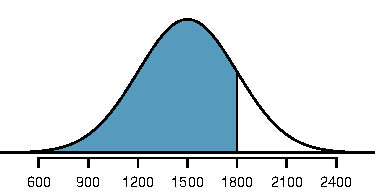
\includegraphics[width=0.5\textwidth]{ch_distributions_oi_biostat/figures/satBelow1800/satBelow1800}
	\caption{The normal model for SAT scores, with shaded area representing scores below 1800.}
	\label{satBelow1800}
\end{figure}
		
\begin{exercisewrap}
\begin{nexercise}
Determine the proportion of SAT test takers who scored better than Student A on the SAT.\footnotemark{}
\end{nexercise}
\end{exercisewrap}
\footnotetext{If 84\% had lower scores than Student A, the number of people who had better scores must be 16\%.}


\textD{\newpage}


\subsection{Normal probability examples}

There are two main types of problems that involve the normal distribution: calculating probabilities from a given value (whether $X$ or $Z$), or identifying the observation that corresponds to a particular probability. 

\begin{examplewrap}
\begin{nexample}{Cumulative SAT scores are well-approximated by a normal model, $N(1500, 300)$. What is the probability that a randomly selected test taker scores at least 1630 on the SAT?}\label{satAbove1630Exam}%	
For any normal probability problem, it can be helpful to start out by drawing the normal curve and shading the area of interest.

\begin{center}
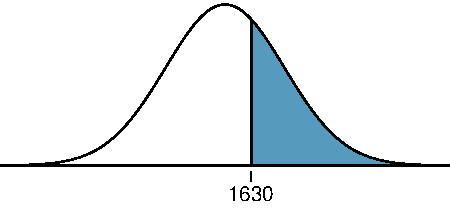
\includegraphics[width=0.45\textwidth]{ch_distributions_oi_biostat/figures/satAbove1630/satAbove1630}
\end{center}
To find the shaded area under the curve, convert 1630 to a Z-score:
\begin{align*}
Z = \frac{x - \mu}{\sigma} = \frac{1630 - 1500}{300} = \frac{130}{300} = 0.43.
\end{align*}
Look up the percentile of $Z=0.43$ in the normal probability table shown in Figure~\ref{zTableShort} or in Appendix~\vref{normalProbabilityTable}: 0.6664. However, note that the percentile describes those who had a Z-score \emph{lower} than 0.43, or in other words, the area below 0.43. To find the area \emph{above} $Z=0.43$, subtract the area of the lower tail from the total area under the curve, 1:
\begin{center}
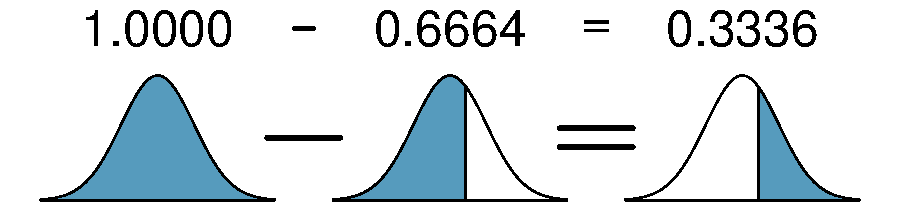
\includegraphics[width=0.5\textwidth]{ch_distributions_oi_biostat/figures/subtractingArea/subtractingArea}
\end{center}
The probability that a student scores at least 1630 on the SAT is 0.3336.
\end{nexample}
\end{examplewrap}

\begin{onebox}{Discrete versus continuous probabilities}
\label{discreteVsContDistr}%
Recall that the probability of a continuous random variable equaling some exact value is always 0. As a result, for a continuous random variable $X$, $P(X \leq x) = P(X < x)$ and $P(X \geq x) = P(X > x)$. It is valid to state that $P(X \geq x) = 1 - P(X \leq x) = 1 - P(X < x)$.\\
		
This is \textit{not} the case for discrete random variables. For example, for a discrete random variable $Y$, $P(Y \geq 2) = 1 - P(Y < 2) = 1 - P(Y \leq 1)$. It would be incorrect to claim that $P(Y \geq 2) = 1 - P(Y \leq 2)$.
\end{onebox}

\begin{exercisewrap}
\begin{nexercise}
What is the probability of a student scoring at most 1630 on the SAT?\footnotemark{}
\end{nexercise}
\end{exercisewrap}
\footnotetext{This probability was calculated as part of Example~\ref{satAbove1630Exam}: 0.6664. A picture for this exercise is represented by the shaded area below ``0.6664'' in Example~\ref{satAbove1630Exam}.}

\begin{exercisewrap}
\begin{nexercise}
Systolic blood pressure for adults 60 years of age and older in the United States is approximately normally distributed: $N(136, 40)$. What is the probability of an adult in this age group having systolic blood pressure of 140 mm Hg or greater?\footnotemark{}
\end{nexercise}
\end{exercisewrap}
\footnotetext{The Z-score for this observation was calculated in Exercise~\ref{nhanes_bp} as 0.1. From the table, the $P(Z \ge 0.1) = 1 - 0.54 = 0.46$.}

\textD{\newpage}

\begin{examplewrap}
\begin{nexample}{The height of adult males in the United States between the ages of 20 and 62 is nearly normal, with mean 70 inches and standard deviation 3.3 inches.\footnotemark{} What is the probability that a random adult male is between 5'9'' and 6'2''?}
	These heights correspond to 69 inches and 74 inches. First, draw the figure. The area of interest is an interval, rather than a tail area.
	\begin{center}
		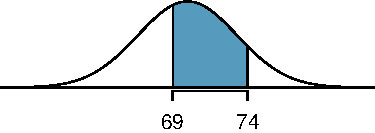
\includegraphics[width=0.43\textwidth]{ch_distributions_oi_biostat/figures/between59And62/between59And62}
	\end{center}
	To find the middle area, find the area to the left of 74; from that area, subtract the area to the left of 69.
	
	First, convert to Z-scores:
	
	\begin{align*}
	Z_{74} = \dfrac{x-\mu}{\sigma} = \dfrac{74-70}{3.3} = 1.21, \qquad Z_{62} = \dfrac{x-\mu}{\sigma} = \dfrac{69-70}{3.3} = -0.30.
	\end{align*}
	
	From the normal probability table, the areas are respectively, $0.8869$ and $0.3821$. The middle area is $0.8869 - 0.3821 = 0.5048$. The probability of being between heights 5'9'' and 6'2'' is 0.5048.
	\begin{center}
		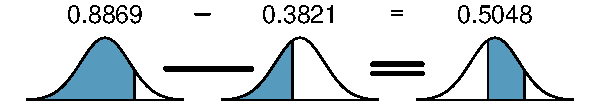
\includegraphics[width=0.65\textwidth]{ch_distributions_oi_biostat/figures/subtracting2Areas/subtracting2Areas}
	\end{center}
\end{nexample}
\end{examplewrap}
\footnotetext{As based on a sample of 100 men, from the USDA Food Commodity Intake Database.}

\begin{exercisewrap}
\begin{nexercise}
What percentage of adults in the United States ages 60 and older have blood pressure between 145 and 130 mm Hg?\footnotemark{}
\end{nexercise}
\end{exercisewrap}
\footnotetext{First calculate Z-scores, then find the percent below 145 mm Hg and below 130 mm Hg: $Z_{145} = 0.23 \to 0.5910$, $Z_{130} = -0.15 \to 0.4404$ (area above). Final answer: $0.5890 - 0.4404 = 0.1486$.}

\textD{\newpage}

\begin{examplewrap}
\begin{nexample}{How tall is a man with height in the 40$^{th}$ percentile?}\label{normalExam40Perc}
First, draw a picture. The lower tail probability is 0.40, so the shaded area must start before the mean. \vspace{-1mm}
\begin{center}
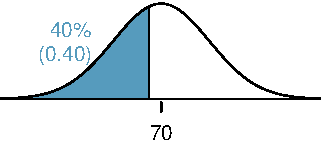
\includegraphics[width=0.35\textwidth]{ch_distributions_oi_biostat/figures/height40Perc/height40Perc}\vspace{-1mm}
\end{center}

Determine the Z-score associated with the $40^{th}$ percentile. Because the percentile is below 50\%, $Z$ will be negative. Look for the probability inside the negative part of table that is closest to 0.40: 0.40 falls in row $-0.2$ and between columns $0.05$ and $0.06$. Since it falls closer to $0.05$, choose $Z=-0.25$.

Convert the Z-score to $X$, where $X \sim N(70, 3.3)$. 
\begin{align*}
X = \mu + \sigma Z = 70 + (-0.25)(3.3) = 69.18.
\end{align*}
A man with height in the 40$^{th}$ percentile is 69.18 inches tall, or about 5' 9''. 
\end{nexample}
\end{examplewrap}

\begin{exercisewrap}
\begin{nexercise}
(a) What is the $95^{th}$ percentile for SAT scores? (b) What is the $97.5^{th}$ percentile of the male heights?\footnotemark{}
\end{nexercise}
\end{exercisewrap}
\footnotetext{(a) Look for 0.95 in the probability portion (middle part) of the normal probability table: row 1.6 and (about) column 0.05, i.e. $Z_{95}=1.65$. Knowing $Z_{95}=1.65$, $\mu = 1500$, and $\sigma = 300$, convert Z to $x$: $1500 + (1.65)(300) = 1995$. (b) Similarly, find $Z_{97.5} = 1.96$, and convert to $x$: $x_{97.5} = 76.5$ inches.}


\textD{\newpage}


\subsection{Normal approximation to the binomial distribution}
	
\index{distribution!binomial!normal approximation|(}

The normal distribution can be used to approximate other distributions, such as the binomial distribution. The binomial formula is cumbersome when sample size is large, particularly when calculating probabilities for a large number of observations. Under certain conditions, the normal distribution can be used to approximate binomial probabilities. This method was widely used when calculating binomial probabilities by hand was the only option. Nowadays, modern statistical software is capable of calculating exact binomial probabilities even for very large $n$. The normal approximation to the binomial is discussed here since it is an important result that will be revisited in later chapters.

Consider the binomial model when probability of success is $p=0.10$. Figure~\ref{fourBinomialModelsShowingApproxToNormal} shows four hollow histograms for simulated samples from the binomial distribution using four different sample sizes: $n=10, 30, 100, 300$. As the sample size increases from $n=10$ to $n=300$, the distribution is transformed from a blocky and skewed distribution into one resembling the normal curve.
	
\begin{figure}[h]
		\centering
		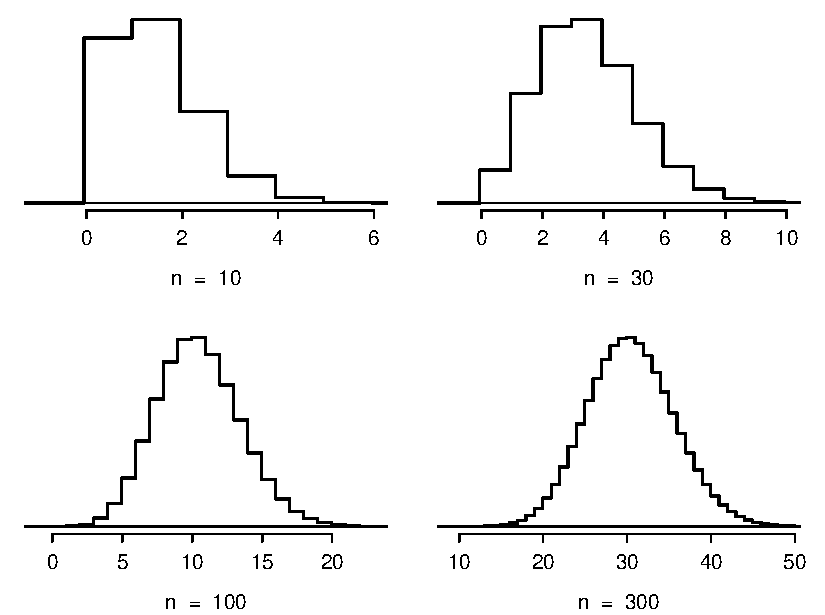
\includegraphics[width=0.83\textwidth]{ch_distributions_oi_biostat/figures/fourBinomialModelsShowingApproxToNormal/fourBinomialModelsShowingApproxToNormal}
		\caption{Hollow histograms of samples from the binomial model when $p=0.10$. The sample sizes for the four plots are $n=10$, 30, 100, and 300, respectively.}
		\label{fourBinomialModelsShowingApproxToNormal}
\end{figure}
	
\begin{onebox}{Normal approximation of the binomial distribution}
The binomial distribution with probability of success $p$ is nearly normal when the sample size $n$ is sufficiently large such that $np$ and $n(1-p)$ are both at least 10. The approximate normal distribution has parameters corresponding to the mean and standard deviation of the binomial distribution:\vspace{-1.5mm}
\begin{align*}
\mu &= np
&&\sigma= \sqrt{np(1-p)}
\end{align*}
\end{onebox}

\begin{examplewrap}
\begin{nexample}{Approximately 20\% of the US population smokes cigarettes. A local government commissioned a survey of 400 randomly selected individuals to investigate whether their community might have a lower smoker rate than 20\%. The survey found that 59 of the 400 participants smoke cigarettes. If the true proportion of smokers in the community is 20\%, what is the probability of observing 59 or fewer smokers in a sample of 400 people?}\label{approxBinomialForN400P20SmokerExample}
		
The desired probability is equivalent to the sum of the individual probabilities of observing $k=0$, 1, ..., 58, or 59 smokers in a sample of $n=400$: $P(X \leq 59)$. Confirm that the normal approximation is valid: $np=400\times 0.20=80$, $n(1-p)=400\times 0.8=320$. To use the normal approximation, calculate the mean and standard deviation from the binomial model:
\begin{align*}
		\mu &= np = 80
		&\sigma &= \sqrt{np(1-p)} = 8.
\end{align*}
		
Convert 59 to a Z-score: $Z = \dfrac{59-80}{8} = -2.63$. Use the normal probability table to identify the left tail area, which is 0.0043. 
		
This estimate is very close to the answer derived from the exact binomial calculation:
\[P(k=0\text{ or }k=1\text{ or }\cdots\text{ or } k=59) = P(k=0) + P(k=1) + \cdots + P(k=59) = 0.0041. \]
\end{nexample}
\end{examplewrap}
	
However, even when the conditions for using the approximation are met, the normal approximation to the binomial tends to perform poorly when estimating the probability of a small range of counts. Suppose the normal approximation is used to compute the probability of observing 69, 70, or 71 smokers in 400 when $p=0.20$. In this setting, the exact binomial and normal approximation result in notably different answers: the approximation gives 0.0476, while the binomial returns 0.0703.
	
The cause of this discrepancy is illustrated in Figure~\ref{normApproxToBinomFail}, which shows the areas representing the binomial probability (outlined) and normal approximation (shaded). Notice that the width of the area under the normal distribution is 0.5 units too slim on both sides of the interval.
	
\begin{figure}[h]
		\centering
		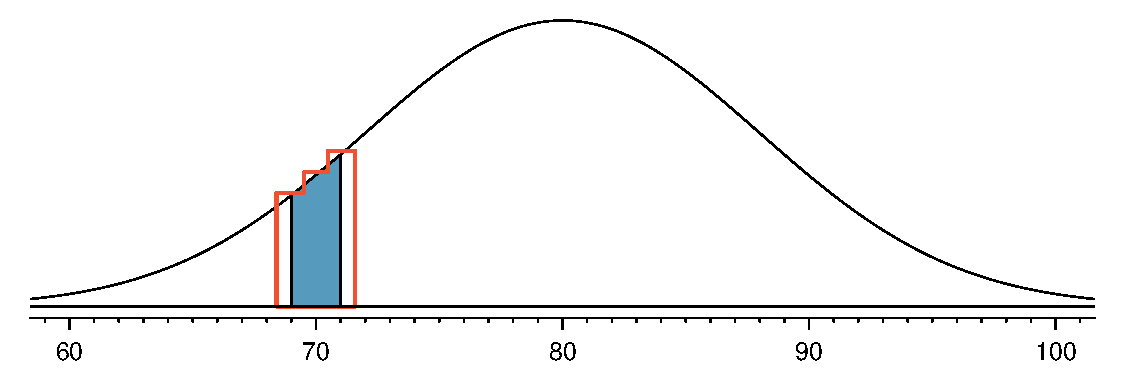
\includegraphics[width=0.77\textwidth]{ch_distributions_oi_biostat/figures/normApproxToBinomFail/normApproxToBinomFail}
		\caption{A normal curve with the area between 69 and 71 shaded. The outlined area represents the exact binomial probability.}
		\label{normApproxToBinomFail}
\end{figure}
	
The normal approximation can be improved if the cutoff values for the range of observations is modified slightly: the lower value should be reduced by 0.5 and the upper value increased by 0.5. The normal approximation with continuity correction gives 0.0687 for the probability of observing 69, 70, or 71 smokers in 400 when $p = 0.20$, which is closer to the exact binomial result of 0.0703. 

This adjustment method is known as a continuity correction, which allows for increased accuracy when a continuous distribution is used to approximate a discrete one. The modification is typically not necessary when computing a tail area, since the total interval in that case tends to be quite wide.
	
\index{distribution!binomial!normal approximation|)}


\subsection{Evaluating the normal approximation}
\label{assessingNormal}

The normal model can also be used to approximate data distributions. While using a normal model can be convenient, it is important to remember that normality is always an approximation. Testing the appropriateness of the normal assumption is a key step in many data analyses.

\index{normal probability plot|(}

\begin{figure}[h]
	\centering
	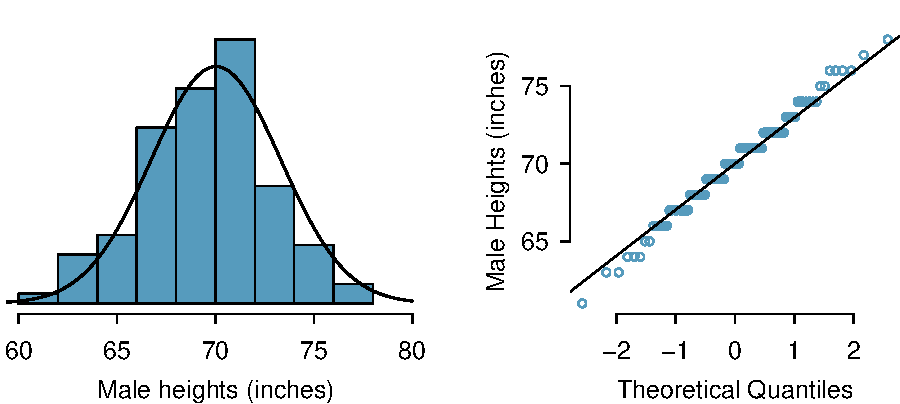
\includegraphics[width=0.8\textwidth]{ch_distributions_oi_biostat/figures/fcidMHeights/fcidMHeights}
	\caption{A sample of 100 male heights. Since the observations are rounded to the nearest whole inch, the points in the normal probability plot appear to jump in increments.}
	\label{fcidMHeights}
\end{figure}

Example~\ref{normalExam40Perc} suggests the distribution of heights of US males is well approximated by the normal model. There are two visual methods used to assess the assumption of normality. The first is a simple histogram with the best fitting normal curve overlaid on the plot, as shown in the left panel of Figure~\ref{fcidMHeights}. The sample mean $\bar{x}$ and standard deviation $s$ are used as the parameters of the best fitting normal curve. The closer this curve fits the histogram, the more reasonable the normal model assumption. More commonly, a \term{normal probability plot} is used, such as the one shown in the right panel of Figure~\ref{fcidMHeights}.\footnote{Also called a \term{quantile-quantile plot}, or Q-Q plot.} If the points fall on or near the line, the data closely follow the normal model.

\textD{\newpage}

\begin{examplewrap}
\begin{nexample}{Three datasets were simulated from a normal distribution, with sample sizes $n = 40$, $n = 100$, and $n = 400$; the histograms and normal probability plots of the datasets are shown in Figure~\ref{normalExamples}. What happens as sample size increases?}\label{normalExamplesExample}%
As sample size increases, the data more closely follows the normal distribution; the histograms become more smooth, and the points on the Q-Q plots show fewer deviations from the line.

It is important to remember that when evaluating normality in a small dataset, apparent deviations from normality may simply be due to small sample size. Remember that all three of these simulated datasets are drawn from a normal distribution.

When assessing the normal approximation in real data, it will be rare to observe a Q-Q plot as clean as the one shown for $n = 400$. Typically, the normal approximation is reasonable even if there are some small observed departures from normality in the tails, such as in the plot for $n = 100$.
\end{nexample}
\end{examplewrap}

\begin{figure}[h]
\centering
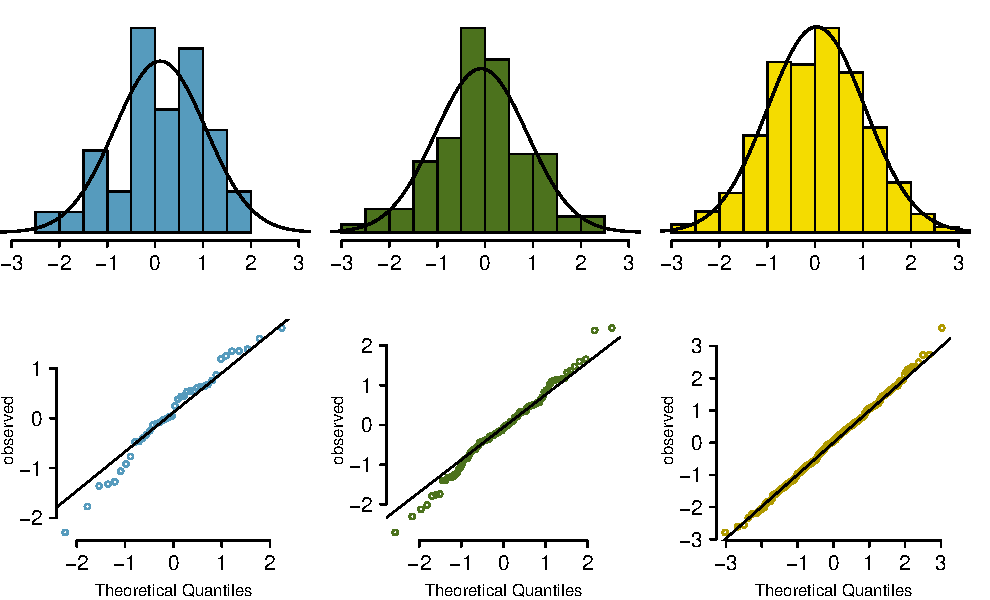
\includegraphics[width=\textwidth]{ch_distributions_oi_biostat/figures/normalExamples/normalExamples}
\caption{Histograms and normal probability plots for three simulated normal data sets; $n=40$ (left), $n=100$ (middle), $n=400$ (right).}
\label{normalExamples}
\end{figure}

\textD{\newpage}

\begin{examplewrap}
\begin{nexample}{Would it be reasonable to use the normal distribution to accurately calculate percentiles of heights of NBA players? Consider all 435 NBA players from the 2008-9 season presented in Figure~\ref{nbaNormal}.\footnotemark{}}
The histogram in the left panel is slightly left skewed, and the points in the normal probability plot do not closely follow a straight line, particularly in the upper quantiles. The normal model is not an accurate approximation of NBA player heights.
\end{nexample}
\end{examplewrap}
\footnotetext{These data were collected from \oiRedirect{textbook-nba_com}{www.nba.com}.}

\begin{figure}[h]
	\centering
	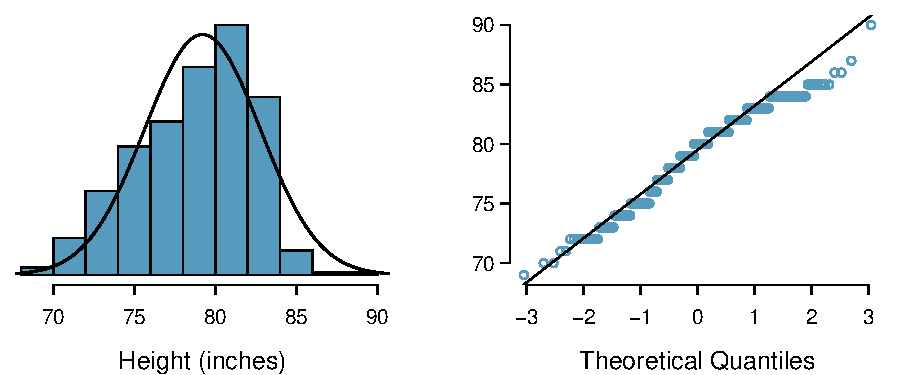
\includegraphics[width=0.80\textwidth]{ch_distributions_oi_biostat/figures/nbaNormal/nbaNormal}
	\caption{Histogram and normal probability plot for the NBA heights from the 2008-9 season.}
	\label{nbaNormal}
\end{figure}		
		
\begin{examplewrap}
\begin{nexample}{Consider the poker winnings of an individual over 50 days. A histogram and normal probability plot of these data are shown in Figure~\ref{pokerNormal} Evaluate whether a normal approximation is appropriate.}
The data are very strongly right skewed\index{skew!example: very strong} in the histogram, which corresponds to the very strong deviations on the upper right component of the normal probability plot. These data show very strong deviations from the normal model; the normal approximation should not be applied to these data.
\end{nexample}
\end{examplewrap}

\begin{figure}[h]
	\centering
	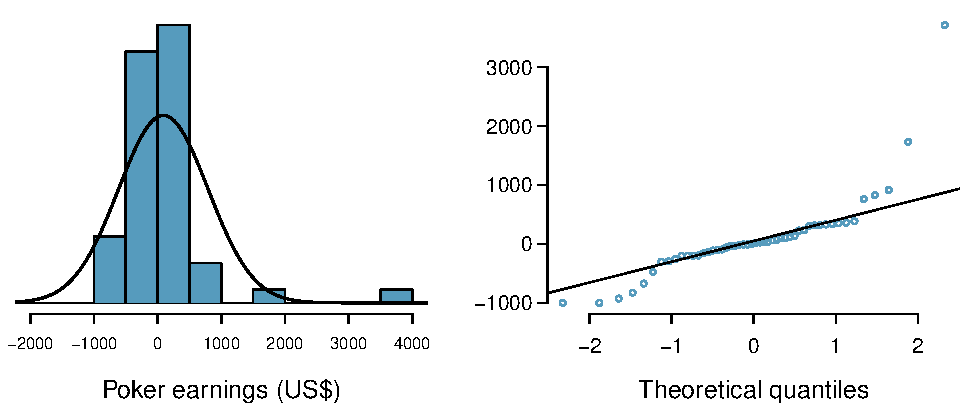
\includegraphics[width=0.85\textwidth]{ch_distributions_oi_biostat/figures/pokerNormal/pokerNormal}
	\caption{A histogram of poker data with the best fitting normal plot and a normal probability plot.}
	\label{pokerNormal}
\end{figure}	

\begin{exercisewrap}
\begin{nexercise}\label{normalQuantileExercise}%
Determine which data sets represented in Figure~\ref{normalQuantileExer} plausibly come from a nearly normal distribution.\footnotemark{}
\end{nexercise}
\end{exercisewrap}
\footnotetext{Answers may vary. The top-left plot shows some deviations in the smallest values in the dataset; specifically, the left tail shows some large outliers. The top-right and bottom-left plots do not show any obvious or extreme deviations from the lines for their respective sample sizes, so a normal model would be reasonable. The bottom-right plot has a consistent curvature that suggests it is not from the normal distribution. From examining the vertical coordinates of the observations, most of the data are between -20 and 0, then there are about five observations scattered between 0 and 70; this distribution has strong right skew.}

\begin{figure}[h]
	\centering
	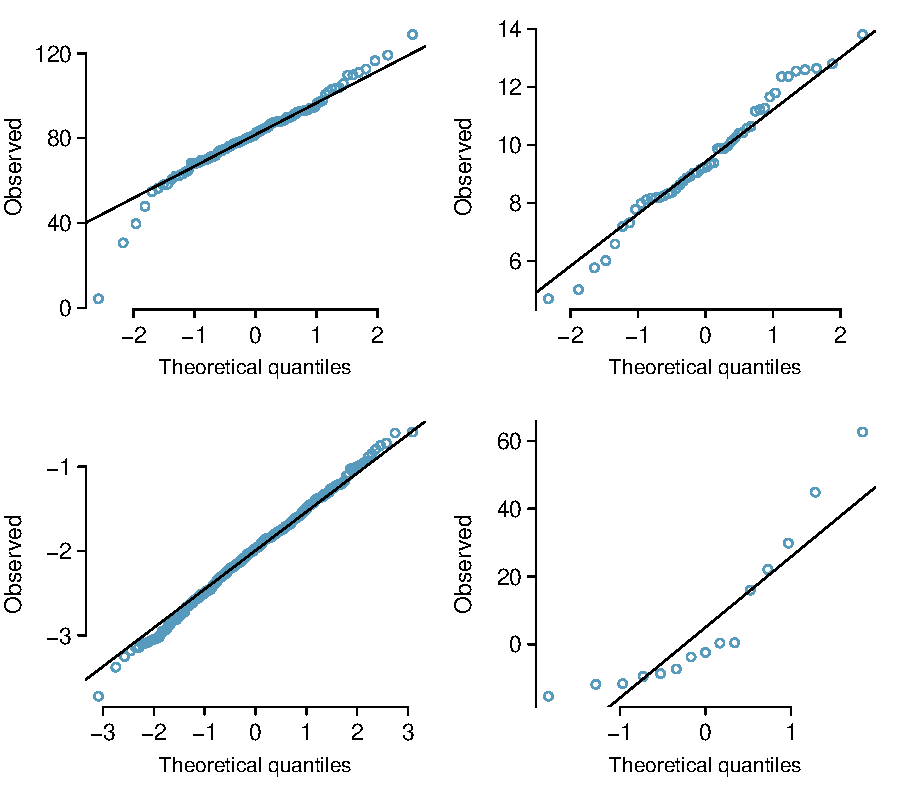
\includegraphics[width=0.80\textwidth]{ch_distributions_oi_biostat/figures/normalQuantileExer/normalQuantileExer}
	\caption{Four normal probability plots for Guided Practice~\ref{normalQuantileExercise}.}
	\label{normalQuantileExer}
\end{figure}

\textD{\newpage}

When observations spike downwards on the left side of a normal probability plot, this indicates that the data have more outliers in the left tail expected under a normal distribution. When observations spike upwards on the right side, the data have more outliers in the right tail than expected under the normal distribution.

\begin{exercisewrap}
\begin{nexercise}\label{normalQuantileExerciseAdditional}%
Figure~\ref{normalQuantileExerAdditional} shows normal probability plots for two distributions that are skewed. One distribution is skewed to the low end (left skewed) and the other to the high end (right skewed). Which is which?\footnotemark{}
\end{nexercise}
\end{exercisewrap}
\footnotetext{Examine where the points fall along the vertical axis. In the first plot, most points are near the low end with fewer observations scattered along the high end; this describes a distribution that is skewed to the high end. The second plot shows the opposite features, and this distribution is skewed to the low end.}

\begin{figure}[h]
\centering
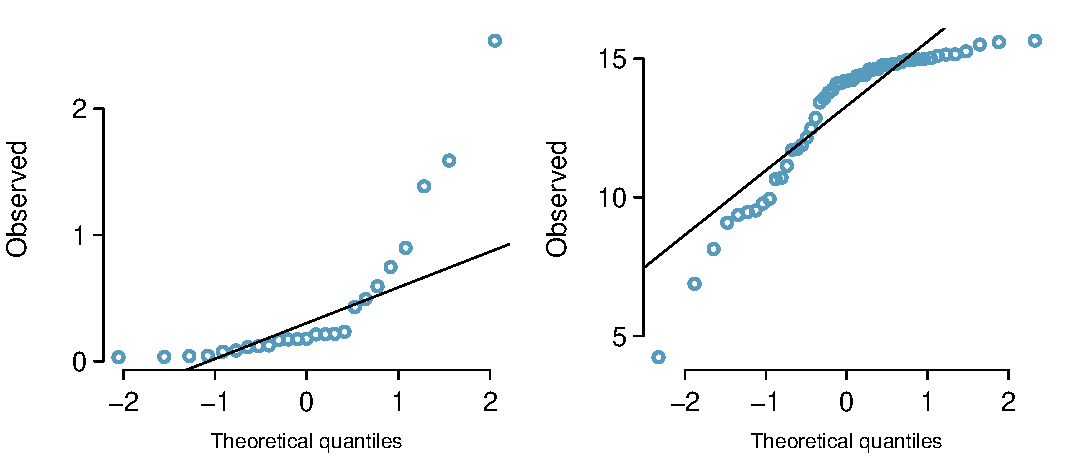
\includegraphics[width=0.80\textwidth]{ch_distributions_oi_biostat/figures/normalQuantileExer/normalQuantileExerAdditional}
\caption{Normal probability plots for Guided Practice~\ref{normalQuantileExerciseAdditional}.}
\label{normalQuantileExerAdditional}
\end{figure}


\index{normal probability plot|)}
\index{distribution!normal|)}


%_________________
\section{Poisson distribution}
\label{poisson}

\index{distribution!Poisson|(}

The \termsub{Poisson distribution}{distribution!Poisson} is a discrete distribution used to calculate probabilities for the number of occurrences of a rare event.  In technical terms, it is used as a model for count data. For example, historical records of hospitalizations in New York City indicate that among a population of approximately 8 million people, 4.4 people are hospitalized each day for an acute myocardial infarction (AMI), on average.  A histogram of showing the distribution of the number of AMIs per day on 365 days for NYC is shown in Figure~\ref{amiIncidencesOver100Days}.\footnote{These data are simulated. In practice, it would be important to check for an association between successive days.}

\begin{figure}[h]
	\centering
	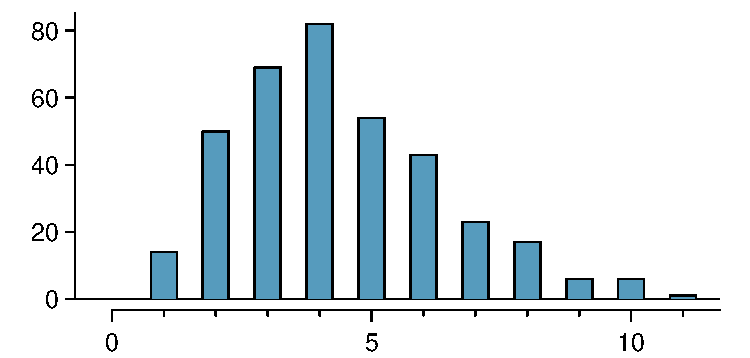
\includegraphics[width=0.7\textwidth]{ch_distributions_oi_biostat/figures/amiIncidencesOver100Days/amiIncidencesOver100Days}
	\caption{A histogram of the number of people hospitalized for an AMI on 365 days for NYC, as simulated from a Poisson distribution with mean 4.4.}
	\label{amiIncidencesOver100Days}
\end{figure}


\begin{onebox}{Poisson distribution}
The Poisson distribution is a probability model for the number of events that occur in a population.  The probability that exactly $k$ events occur is given by 
\begin{align*}
P(X = k) = \frac{e^{-\lambda}(\lambda)^{k}}{k!},
\end{align*}
where $k$ may take a value 0, 1, 2, \dots The mean and standard deviation of this distribution are $\lambda$ and $\sqrt{\lambda}$, respectively.
A Poisson random variable $X$ can be expressed as $X \sim \textrm{Pois}(\lambda)$.
\end{onebox}%
\marginpar[\raggedright\vspace{-35mm}

$\textrm{Pois}(\lambda)$\vspace{1mm}\\\footnotesize Poisson dist.\\with rate $\lambda$]{\raggedright\vspace{-35mm}
	
	$\textrm{Pois}(\lambda)$\vspace{1mm}\\\footnotesize Poisson dist.\\with rate $\lambda$} 

When events accumulate over time in such a way that the probability an event occurs in an interval is proportional to the length of an interval and that the number of events in non-overlapping intervals are independent, the parameter $\lambda$ \marginpar[\raggedright\vspace{-5mm}

$\lambda$\vspace{0mm}\\\footnotesize Rate for the\\Poisson dist.]{\raggedright\vspace{-5mm}
	
	$\lambda$\vspace{0mm}\\\footnotesize Rate for the\\Poisson dist.}\index{Greek!lambda@lambda ($\lambda$)} (the Greek letter \textit{lambda}) represents the average number of events per unit time; i.e., the rate per unit time.

In this setting, the number of events in $t$ units of time has probability
\[P(X = k) = \frac{e^{-\lambda t}(\lambda t)^{k}}{k!}, \]
where $k$ takes on values 0, 1, 2, \dots.  When used this way, the mean and standard deviation  are $\lambda t$ and $\sqrt{\lambda t}$, respectively. The rate parameter $\lambda$ represents the expected number of events per unit time, while the quantity $\lambda t$ represents the expected number events over a time period of $t$ units.

The histogram in Figure~\ref{amiIncidencesOver100Days} approximates a Poisson distribution with rate equal to 4.4 events per day, for a population of 8 million. 

\textD{\newpage}

\begin{examplewrap}
\begin{nexample}{In New York City, what is the probability that 2 individuals are hospitalized for AMI in seven days, if the rate is known to be 4.4 deaths per day?}
From the given information, $\lambda = 4.4$, $k = 2$, and $t = 7$. 
\begin{align*}
P(X = k) =& \frac{e^{-\lambda t}(\lambda t)^{k}}{k!} \\
P(X = 2) =& \frac{e^{-4.4 \times 7}(4.4 \times 7)^{2}}{2!} = 1.99 \times 10^{-11}.
\end{align*}
\end{nexample}
\end{examplewrap}

\begin{exercisewrap}
\begin{nexercise}
In New York City, what is the probability that (a) at most 2 individuals are hospitalized for AMI in seven days, (b) at least 3 individuals are hospitalized for AMI in seven days?\footnotemark{}
\end{nexercise}
\end{exercisewrap}
\footnotetext{(a) $P(X \leq 2) = P(X=0) + P(X=1) + P(X=2) = \frac{e^{-4.4 \times 7}(4.4 \times 7)^{0}}{0!} + \frac{e^{-4.4 \times 7}(4.4 \times 7)^{1}}{1!} + \frac{e^{-4.4 \times 7}(4.4 \times 7)^{2}}{2!} = 2.12 \times 10^{-11}$ (b) $P(X \geq 3) = 1 - P(X < 3) = 1 - P(X \leq 2) = 1 - 2.12 \times 10^{-11} \approx 1 $}

A rigorous set of conditions for the Poisson distribution is not discussed here. Generally, the Poisson distribution is used to calculate probabilities for rare events that accumulate over time, such as the occurrence of a disease in a population.

\begin{examplewrap}
\begin{nexample}{For children ages 0 - 14, the incidence rate of acute lymphocytic leukemia (ALL) was approximately 30 diagnosed cases per million children per year in 2010. Approximately 20\% of the US population of 319,055,000 are in this age range. What is the expected number of cases of ALL in the US over five years?}

The incidence rate for one year can be expressed as $30/1,000,000 = 0.00003$; for five years, the rate is $(5)(0.00003) = 0.00015$. The number of children age 0-14 in the population is $(0.20)(319,055,000) \approx 63,811,000$. 
\begin{align*}
\lambda &= \text{(relevant population size)(rate per child)} \\
&= 63,811,000 \times 0.00015 \\
&= 9,571.5
\end{align*}
	
The expected number of cases over five years is 9,571.5 cases.
\end{nexample}
\end{examplewrap}

\index{distribution!Poisson|)}


%_________________
\section{Distributions related to Bernoulli trials}
\label{distRelatedToBernoulli}

The binomial distribution is not the only distribution that can be built from a series of repeated Bernoulli trials. This section discusses the geometric, negative binomial, and hypergeometric distributions.

\subsection{Geometric distribution}
\label{geomDist}

\index{distribution!geometric|(}

The geometric distribution describes the waiting time until one success for a series of independent Bernoulli random variables, in which the probability of success $p$ remains constant.

\begin{examplewrap}
\begin{nexample}{Recall that in the Milgram shock experiments, the probability of a person refusing to give the most severe shock is $p = 0.35$. Suppose that participants are tested one at a time until one person refuses; i.e., until the first occurrence of a successful trial. What are the chances that the first occurrence happens with the first trial? The second trial? The third?}\label{waitForShocker}%
The probability that the first trial is successful is simply $p = 0.35$. 

If the second trial is the first successful one, then the first one must have been unsuccessful. Thus, the probability is given by $(0.65)(0.35) = 0.228$.

Similarly, the probability that the first success is the third trial: $(0.65)(0.65)(0.35) = 0.148$.

This can be stated generally. If the first success is on the $n^{th}$ trial, then there are $n-1$ failures and finally 1 success, which corresponds to the probability $(0.65)^{n-1}(0.35)$.
\end{nexample}
\end{examplewrap}

The geometric distribution from Example~\ref{waitForShocker} is shown in Figure~\ref{geometricDist35}. In general, the probabilities for a geometric distribution decrease \term{exponentially}.

\begin{figure}[h]
\centering
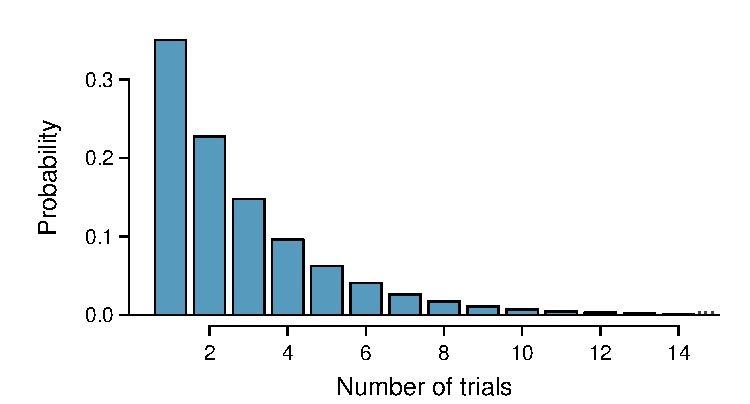
\includegraphics[width=0.8\textwidth]{ch_distributions_oi_biostat/figures/geometricDist35/geometricDist35}
\caption{The geometric distribution when the probability of success is \mbox{$p=0.35$}.}
\label{geometricDist35}
\end{figure}

\begin{onebox}{Geometric Distribution}\index{distribution!geometric|textbf}
If the probability of a success in one trial is $p$ and the probability of a failure is $1-p$, then the probability of finding the first success in the $k^{th}$ trial is given by
\begin{eqnarray*}
P(X = k) = (1-p)^{k-1}p.
\end{eqnarray*}
The mean (i.e. expected value), variance, and standard deviation of this wait time are given by
\begin{align*}
\mu &= \frac{1}{p}
	&\sigma^2&=\frac{1-p}{p^2}
	&\sigma &= \sqrt{\frac{1-p}{p^2}}
\label{geomFormulas}
\end{align*}
A geometric random variable $X$ can be expressed as $X \sim \textrm{Geom}(p)$.
\end{onebox}

\marginpar[\raggedright\vspace{-45mm}

$\textrm{Geom}(p)$\vspace{1mm}\\\footnotesize Geometric dist.\\with $p$ prob. of success]{\raggedright\vspace{-45mm}
	
	$\textrm{Geom}(p)$\vspace{1mm}\\\footnotesize Geometric dist.\\with $p$ prob. of success} 

\begin{exercisewrap}
\begin{nexercise}
If individuals were examined until one did not administer the most severe shock, how many might need to be tested before the first success?\footnotemark{}
\end{nexercise}
\end{exercisewrap}
\footnotetext{About $1/p = 1/0.35 = 2.86$ individuals.}

\begin{examplewrap}
\begin{nexample}{What is the probability of the first success occurring within the first 4 people?}\label{marglimFirstSuccessIn4}%
This is the probability it is the first ($k=1$), second ($k=2$), third ($k=3$), or fourth ($k=4$) trial that is the first success, which represent four disjoint outcomes. Compute the probability of each case and add the separate results:
\begin{eqnarray*}
&&P(X=1, 2, 3,\text{ or }4) \\
	&& \quad = P(X=1)+P(X=2)+P(X=3)+P(X=4) \\
	&& \quad = (0.65)^{1-1}(0.35) + (0.65)^{2-1}(0.35) + (0.65)^{3-1}(0.35) + (0.65)^{4-1}(0.35) \\
	&& \quad = 0.82.
\end{eqnarray*}

Alternatively, find the complement of P(X = 0), since the described event is the complement of no success in 4 trials: $1 - (0.65)^{4}(0.35)^{0} = 0.82$.

There is a 0.82 probability that the first success occurs within 4 trials.
\end{nexample}
\end{examplewrap}

Note that there are differing conventions for defining the geometric distribution; while this text uses the definition that the distribution describes the total number of trials \textit{including} the success, others define the distribution as the number of trials required before the success is obtained. In \textsf{R}, the latter definition is used. 

\index{distribution!geometric|)}


\textD{\newpage}


\subsection{Negative binomial distribution}
\label{negativeBinomial}

\index{distribution!negative binomial|(}

The geometric distribution describes the probability of observing the first success on the $k^{th}$ trial. The \termsub{negative binomial distribution}{distribution!negative binomial} is more general: it describes the probability of observing the $r^{th}$ success on the $k^{th}$ trial.

Suppose a research assistant needs to successfully extract RNA from four plant samples before leaving the lab for the day. Yesterday, it took 6 attempts to attain the fourth successful extraction. The last extraction must have been a success; that leaves three successful extractions and two unsuccessful ones that make up the first five attempts. There are ten possible sequences, which are shown in \ref{successFailureOrdersForRNAExtractions}. 

\begin{figure}[ht]
	\newcommand{\succObs}[1]{{\color{oiB}$\stackrel{#1}{S}$}}
	\centering
	\begin{tabular}{c|c ccc cl | r}
		\multicolumn{8}{c}{\hspace{10mm}Extraction Attempt} \\
		& & 1 & 2 & 3 & 4 & \multicolumn{2}{l}{5\hfill6} \\
		\hline
		1&& $F$ & $F$ & \succObs{1} & \succObs{2} & \succObs{3} & \succObs{4} \\
		2&& $F$ & \succObs{1} & $F$ & \succObs{2} & \succObs{3} & \succObs{4} \\
		3&& $F$ & \succObs{1} & \succObs{2} & $F$ & \succObs{3} & \succObs{4} \\
		4&& $F$ & \succObs{1} & \succObs{2} & \succObs{3} & $F$ & \succObs{4} \\
		5&& \succObs{1} & $F$ & $F$ & \succObs{2} & \succObs{3} & \succObs{4} \\
		6&& \succObs{1} & $F$ & \succObs{2} & $F$ & \succObs{3} & \succObs{4} \\
		7&& \succObs{1} & $F$ & \succObs{2} & \succObs{3} & $F$ & \succObs{4} \\
		8&& \succObs{1} & \succObs{2} & $F$ & $F$ & \succObs{3} & \succObs{4} \\
		9&& \succObs{1} & \succObs{2} & $F$ & \succObs{3} & $F$ & \succObs{4} \\
		10&& \succObs{1} & \succObs{2} & \succObs{3} & $F$ & $F$ & \succObs{4} \\
	\end{tabular}
	\caption{The ten possible sequences when the fourth successful extraction is on the sixth attempt.}
	\label{successFailureOrdersForRNAExtractions}
\end{figure}

\begin{exercisewrap}
\begin{nexercise}\label{probOfEachSeqOfSixTriesToGetFourSuccesses}%
Each sequence in Figure~\ref{successFailureOrdersForRNAExtractions} has exactly two failures and four successes with the last attempt always being a success. If the probability of a success is $p=0.8$, find the probability of the first sequence.\footnotemark{}
\end{nexercise}
\end{exercisewrap}
\footnotetext{The first sequence: $0.2\times0.2\times0.8\times0.8\times0.8\times0.8 = 0.0164$.}

If the probability of a successful extraction is $p=0.8$, what is the probability that it takes exactly six attempts to reach the fourth successful extraction? As expressed by \ref{probOfEachSeqOfSixTriesToGetFourSuccesses}, there are 10 different ways that this event can occur. The probability of the first sequence was identified in Guided Practice~\ref{probOfEachSeqOfSixTriesToGetFourSuccesses} as 0.0164, and each of the other sequences have the same probability. Thus, the total probability is $(10)(0.0164) = 0.164$.

\textD{\newpage}

A general formula for computing a negative binomial probability can be generated using similar logic as for binomial probability. The probability is comprised of two pieces: the probability of a single sequence of events, and then the number of possible sequences. The probability of observing $r$ successes out of $k$ attempts can be expressed as $(1-p)^{k-r} p^{r}$. Next, identify the number of possible sequences. In the above example, 10 sequences were identified by fixing the last observation as a success and looking for ways to arrange the other observations. In other words, the goal is to arrange $r-1$ successes in $k-1$ trials. This can be expressed as: \[{k-1 \choose r-1} = \frac{(k-1)!}{(r-1)! \left((k-1) - (r-1)\right)!} = \frac{(k-1)!}{(r-1)! \left(k - r\right)!}.\]

\begin{onebox}{Negative binomial distribution}
The negative binomial distribution describes the probability of observing the $r^{th}$ success on the $k^{th}$ trial, for independent trials:
\begin{eqnarray}
P(X = k) = {k-1 \choose r-1} p^{r}(1-p)^{k-r},
\label{negativeBinomialEquation}
\end{eqnarray}
where $p$ is the probability an individual trial is a success.

The mean and variance are given by\vspace{-2.5mm}
\begin{align*}
\mu &= \frac{r}{p}
&\sigma^2&=\frac{r(1-p)}{p^2}
\end{align*}
A negative binomial random variable $X$ can be expressed as $X \sim \textrm{NB}(r, p)$.
\end{onebox}

\marginpar[\raggedright\vspace{-45mm}

$\textrm{NB}(r, p)$\vspace{1mm}\\\footnotesize Neg. Bin. dist.\\with $r$ successes\\\& $p$ prob. of success]{\raggedright\vspace{-45mm}
	
	$\textrm{NB}(r, p)$\vspace{1mm}\\\footnotesize Neg. Bin. dist.\\with $k$ successes\\\& $p$ prob. of success} 

\begin{onebox}{Is it negative binomial? Four conditions to check.}
(1) The trials are independent. \\
(2) Each trial outcome can be classified as a success or failure. \\
(3) The probability of a success ($p$) is the same for each trial. \\
(4) The last trial must be a success.
\end{onebox}


\begin{examplewrap}
\begin{nexample}{Calculate the probability of a fourth successful extraction on the fifth attempt.}
The probability of a single success is $p=0.8$, the number of successes is $r=4$, and the number of necessary attempts under this scenario is $k=5$.
\begin{align*}
{k-1 \choose r-1}p^r(1-p)^{k-r}\ 
	=\ \frac{4!}{3!1!} (0.8)^4 (0.2)\ 
	=\ 4 \times 0.08192\ 
	=\ 0.328.
\end{align*}
\end{nexample}
\end{examplewrap}

\textD{\newpage}

\begin{exercisewrap}
\begin{nexercise}
Assume that each extraction attempt is independent. What is the probability that the fourth success occurs within 5 attempts?\footnotemark{}
\end{nexercise}
\end{exercisewrap}
\footnotetext{If the fourth success ($r=4$) is within five attempts, it either took four or five tries ($k=4$ or $k=5$):
\begin{align*}
& P(k=4\text{ OR }k=5) = P(k=4) + P(k=5) \\
&\quad = {4-1 \choose 4-1} 0.8^4 + {5-1 \choose 4-1} (0.8)^4(1-0.8) = 1\times 0.41 + 4\times 0.082 = 0.41 + 0.33 = 0.74.
\end{align*}}

\begin{onebox}{Binomial versus negative binomial}
The binomial distribution is used when considering the number of successes for a fixed number of trials. For negative binomial problems, there is a fixed number of successes and the goal is to identify the number of trials necessary for a certain number of successes (note that the last observation must be a success).
\end{onebox}

\begin{exercisewrap}
\begin{nexercise}
On 70\% of days, a hospital admits at least one heart attack patient. On 30\% of the days, no heart attack patients are admitted. Identify each case below as a binomial or negative binomial case, and compute the probability. (a) What is the probability the hospital will admit a heart attack patient on exactly three days this week? (b) What is the probability the second day with a heart attack patient will be the fourth day of the week? (c) What is the probability the fifth day of next month will be the first day with a heart attack patient?\footnotemark{}
\end{nexercise}
\end{exercisewrap}
\footnotetext{In each part, $p=0.7$. (a) The number of days is fixed, so this is binomial. The parameters are $k=3$ and $n=7$: 0.097. (b) The last "success" (admitting a patient) is fixed to the last day, so apply the negative binomial distribution. The parameters are $r=2$, $k=4$: 0.132. (c) This problem is negative binomial with $r=1$ and $k=5$: 0.006. Note that the negative binomial case when $r=1$ is the same as using the geometric distribution.}

In \textsf{R}, the negative binomial distribution is defined as the number of failures that occur before a target number of successes is reached; i.e., $k - r$. In this text, the distribution is defined in terms of the total number of trials required to observe $r$ successes, where the last trial is necessarily a success. 

\index{distribution!negative binomial|)}


\textD{\newpage}


\subsection{Hypergeometric distribution}
\label{hypergeometric}

\index{distribution!hypergeometric|(}

Suppose that a large number of deer live in a forest. Researchers are interested in using the capture-recapture method to estimate total population size. A number of deer are captured in an initial sample and marked, then released; at a later time, another sample of deer are captured, and the number of marked and unmarked deer are recorded.\footnote{It is assumed that enough time has passed so that the marked deer redistribute themselves in the population, and that marked and unmarked deer have equal probability of being captured in the second sample.} An estimate of the total population can be calculated based on the assumption that the proportion of marked deer in the second sample should equal the proportion of marked deer in the entire population. For example, if 50 deer were initially captured and marked, and then 5 out of 40 deer (12.5\%) in a second sample are found to be marked, then the population estimate is 400 deer, since 50 out of 400 is 12.5\%.

The capture-recapture method sets up an interesting scenario that requires a new probability distribution. Let $N$ represent the total number of deer in the forest, $m$ the number of marked deer captured in the original sample, and $n$ the number of deer in the second sample. What are the probabilities of obtaining $0, 1, ... , m$ marked deer in the second sample, if $N$ and $m$ are known?

It is helpful to think in terms of a series of Bernoulli trials, where each capture in the second sample represents a trial; consider the trial a success if a marked deer is captured, and a failure if an unmarked deer is captured. If the deer were sampled \textit{with replacement}, such that one deer was sampled, checked if it were marked versus unmarked, then released before another deer was sampled, then the probability of obtaining some number of marked deer in the second sample would be binomially distributed with probability of success $m/N$ (out of $n$ trials). The trials are independent, and the probability of success remains constant across trials.

However, in capture-recapture, the goal is to collect a representative sample such that the proportion of marked deer in the sample can be used to estimate the total population\textemdash the sampling is done \textit{without replacement}. Once a trial occurs and a deer is sampled, it is not returned to the population before the next trial. The probability of success is not constant from trial to trial; i.e., these trials are dependent. For example, if a marked deer has just been sampled, then the probability of sampling a marked deer in the next trial decreases, since there is one fewer marked deer available. 

Suppose that out of 9 deer, 4 are marked. What is the probability of observing 1 marked deer in a sample of size 3, if the deer are sampled without replacement? First, consider the total number of ways to draw 3 deer from the population; As shown in Figure~\ref{hGeomSchematic}, samples may consist of 3, 2, 1, or 0 marked deer. There are ${4 \choose 3}$ ways to obtain a sample consisting of 3 marked deer out of the 4 total marked deer. By independence, there are ${4 \choose 2} {5 \choose 1}$ ways to obtain a sample consisting of exactly 2 marked deer and 1 unmarked deer. In total, there are 84 possible combinations; this quantity is equivalent to ${9 \choose 3}$. Only ${4 \choose 1} {5 \choose 2} = 40$ of those combinations represent the desired event of exactly 1 marked deer. Thus, the probability of observing 1 marked deer in a sample of size 3, under sampling without replacement, equals $40/84 = 0.476$.

\begin{figure}[h]
	\centering
	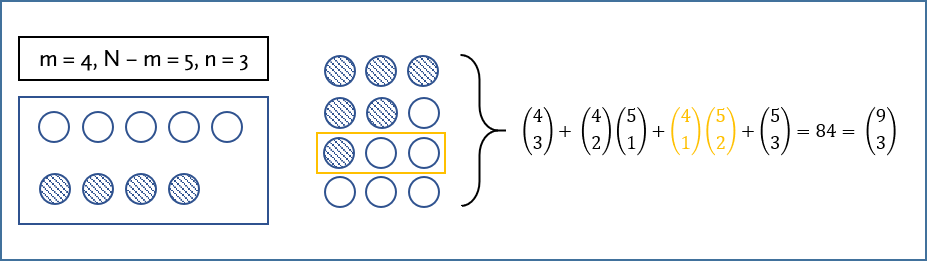
\includegraphics[width=0.880\textwidth]
	{ch_distributions_oi_biostat/figures/hGeomSchematic/hGeomSchematic.png}
	\caption{Possible samples of marked and unmarked deer in a sample $n = 3$, where $m = 4$ and $N - m = 5$. Striped circles represent marked deer, and empty circles represent unmarked deer.}
	\label{hGeomSchematic}
\end{figure}

\textD{\newpage}

\begin{exercisewrap}
\begin{nexercise}
Suppose that out of 9 deer, 4 are marked. What is the probability of observing 1 marked deer in a sample of size 3, if the deer are sampled with replacement?\footnotemark{}
\end{nexercise}
\end{exercisewrap}
\footnotetext{Let $X$ represent the number of marked deer in the sample of size 3. If the deer are sampled with replacement, $X \sim \textrm{Bin}(3, 4/9)$, and $P(X = 1) = { 3 \choose 1 } (4/9)^1 (5/9)^2 = 0.412$.}

\begin{onebox}{Hypergeometric distribution}
The hypergeometric distribution describes the probability of observing $k$ successes in a sample of size $n$, from a population of size $N$, where there are $m$ successes, and individuals are sampled without replacement:
\begin{align*}
P(X = k) = \dfrac{{m \choose k} {N - m \choose n-k}}{{N \choose n}}.
\label{hypergeometricEquation}
\end{align*}

Let $p = m/N$, the probability of success. The mean and variance are given by\vspace{-2.5mm}
\begin{align*}
\mu &= np
&\sigma^2&=np(1-p)\frac{N-n}{N-1}
\end{align*}
A hypergeometric random variable $X$ can be written as $X \sim \textrm{HGeom}(m, N-m, n)$.
\end{onebox}

\begin{onebox}{Is it hypergeometric? Three conditions to check.}
(1) The trials are dependent. \\
(2) Each trial outcome can be classified as a success or failure. \\
(3) The probability of a success is different for each trial.
\end{onebox}

\begin{exercisewrap}
\begin{nexercise}
A small clinic would like to draw a random sample of 10 individuals from their patient list of 120, of which 30 patients are smokers. (a) What is the probability of 6 individuals in the sample being smokers? (b) What is the probability that at least 2 individuals in the sample smoke?\footnotemark{}
\end{nexercise}
\end{exercisewrap}
\footnotetext{(a) Let $X$ represent the number of smokers in the sample. $P(X = 6) = \dfrac{{30 \choose 6}{90 \choose 4}}{{120 \choose 10}} = 0.013$. (b) $P(X \geq 2) = 1 - P(X \leq 1) = 1 - P(X = 0) - P(X = 1) = 1 - \dfrac{{30 \choose 0}{90 \choose 10}}{{120 \choose 10}} - \dfrac{{30 \choose 1}{90 \choose 9}}{{120 \choose 10}} = 0.768$. }

\index{distribution!hypergeometric|)}


%____________
\section{Distributions for pairs of random variables}
\label{correlatedRVs}

\index{joint distribution for random variables|(}
\index{marginal distribution for random variables|(}
\index{conditional distribution for random variables|(}

Example~\ref{sdHealthCostsPartners} calculated the variability in health care costs for an employee and her partner relying on the assumption that the number of health episodes between the two are not related. It could be reasonable to assume that the health status of one person gives no information about the other's health, given that the two are not physically related and were not previously living together. However, associations between random variables can be subtle. For example, couples are often attracted to each other because of common interests or lifestyles, which suggests that health status may actually be related.

The relationship between a pair of discrete random variables is a feature of the \term{joint distribution} of the pair. In this example the joint distribution of annual costs is a table of all possible combinations of costs for the employee and her partner, using the probabilities and costs from the last 10 years (these costs were previously calculated in Example~\ref{example:healthCareCosts}
and Guided Practice~\ref{healthCareCostsPartner}). Entries in the table are probabilities of pairs of annual costs. For example, the entry 0.25 in the second row and second column of Figure~\ref{table:healthExpensesJointDistribution} indicates that in approximately 25\% of the last 10 years, the employee paid \$1,008 in costs while her partner paid \$988.
\begin{figure}[h]
	\centering
	\begin{tabular}{crr}
		\hline
		&   \multicolumn{2}{c}{\textbf{Partner costs, $Y$}} \\
		\textbf{Employee costs, $X$} & \textbf{\$968} & \textbf{\$988} \\ 
		\hline
		\textbf{\$968} & 0.18 & 0.12 \\ 
		\textbf{\$1,008} & 0.15 & 0.25 \\ 
		\textbf{\$1,028}  & 0.04 & 0.16 \\ 
		\textbf{\$1,108}  & 0.03 & 0.07 \\ 
		\hline
	\end{tabular}
	\caption{Joint distribution of health care costs.} 
	\label{table:healthExpensesJointDistribution}
\end{figure}

More generally, the definition of a joint distribution for a pair of random variables $X$ and $Y$ uses the notion of joint probabilities discussed in Section~\ref{marginalAndJointProbabilities}.

\begin{onebox}{Joint distribution}
The \term{joint distribution} $p_{X, Y}(x, y)$ for a pair of random variables $(X, Y)$ is the collection of probabilities
\begin{align*}
p(x_i,y_j) = P(X=x_i \text{ and } Y = y_j)
\end{align*}
for all pairs of values $(x_i,y_j)$ that the random variables $X$ and $Y$ take on.
\end{onebox}

\textD{\newpage}

Joint distributions are often displayed in tabular form as in Figure~\ref{table:healthExpensesJointDistribution}.  If $X$ and $Y$ have $k_1$ and $k_2$ possible values respectively, there will be $(k_1)(k_2)$ possible $(x,y)$ pairs. This is unlike pairs of values $(x,y)$ observed in a dataset, where each observed value of $x$ is usually paired with only one value of $y$. A joint distribution is often best displayed as a table of probabilities, with $(k_1)(k_2)$ entries.  Figure~\ref{table:generalJointDistribution} shows the general form of the table for the joint distribution of two discrete distributions.

\begin{figure}[h]
	\centering
	\begin{tabular}{ccccc}
		\hline
		& \multicolumn{4}{c}{\textbf{Values of $Y$}} \\
		\hline
		\textbf{Values of $X$} & $y_1$ & $y_2$ & $\cdots$ & $y_{k_2}$ \\
		$x_1$ &   $p(x_1, y_1)$ &   $p(x_1, y_2)$  & $\cdots$  & $p(x_1, y_{k_2})$  \\
		$x_2$ &  $p(x_2, y_1)$   &  $p(x_2, y_2)$  & $\cdots$ &   $p(x_2, y_{k_2})$ \\
		$\vdots$ &   $\cdots$  &  $\cdots$  &  $\cdots$ &   $\cdots$ \\
		$x_{k_1}$ & $p(x_{k_1}, y_1)$ &  $p(x_{k_1}, y_2)$  &  $\cdots$ & $p(x_{k_1}, y_{k_2})$\vspace{1.5mm} \\
		\hline
	\end{tabular}
	\caption{Table for a joint distribution. Entries are probabilities for pairs ($x_i, y_j$). These probabilities can be written as $p(x_i, y_j)$ or more specifically, $p_{X, Y}(x_i, y_j)$.}
	\label{table:generalJointDistribution}
\end{figure}

When two variables $X$ and $Y$ have a joint distribution, the \term{marginal distribution} of $X$ is the collection of probabilities for $X$ when $Y$ is ignored.\footnote{The marginal distribution of $X$ can be written as $p_X(x)$, and a specific value in the marginal distribution written as $p_X(x_i)$.}  If $X$ represents employee costs and $Y$ represents partner costs, the event $(X = \$968)$ consists of the two  disjoint events $(X = \$968, Y = \$968)$ and $(X = \$968, Y = \$988)$, so $P(X = \$968) = 0.18 + 0.12 = 0.30$, the sum of the first row of the table. The row sums are the values of the marginal distribution of $X$, while the column sums are the values of the marginal distributions of $Y$. The marginal distributions of $X$ and $Y$ are shown in Figure~\ref{healthExpensesJointMarginalDistribution}, along with the joint distribution of $X$ and $Y$. The term marginal distribution is apt in this setting---the marginal probabilities appear in the table margins.

\begin{figure}[h]
	\centering
	\begin{tabular}{c|rr | c}
		&   \multicolumn{2}{c}{\textbf{Partner Costs, $Y$}} & \\
		\hline
		\textbf{Employee costs, $X$} & \textbf{\$968} & \textbf{\$988} &  \textbf{Marg. Dist., $X$} \\ 
		\hline
		\textbf{\$968} & 0.18 & 0.12 & 0.30\\ 
		\textbf{\$1,008} & 0.15 & 0.25 & 0.40 \\ 
		\textbf{\$1,028}  & 0.04 & 0.16 & 0.20\\ 
		\textbf{\$1,108}  & 0.03 & 0.07  & 0.10\\ 
		\hline
		\textbf{Marg. Dist., $Y$} & 0.40 & 0.60 & 1.00 \\
	\end{tabular}
	\caption{Joint and marginal distributions of health care costs} 
	\label{healthExpensesJointMarginalDistribution}
\end{figure}

For a pair of random variables $X$ and $Y$, the \term{conditional distribution} of $Y$ given a value $x$ of the variable $X$ is the probability distribution of $Y$ when its values are restricted to the value $x$ for $X$. Just as marginal and joint probabilities are used to calculate conditional probabilities, joint and marginal distributions can be used to obtain conditional distributions. If information is observed about the value of one of the correlated random variables, such as $X$, then this information can be used to obtain an updated distribution for $Y$; unlike the marginal distribution of $Y$, the conditional distribution of $Y$ given $X$ accounts for information from $X$.

\textD{\newpage}

\begin{onebox}{Conditional distribution}
The \term{conditional distribution} $p_{Y|X}(y|x)$ for a pair of random variables $(X, Y)$ is the collection of probabilities
\begin{align*}
P(Y = y_j| X = x_i) = \dfrac{P(Y = y_j \text{ and } X = x_i)}{P(X = x_j)}
\end{align*}
for all pairs of values $(x_i,y_j)$ that the random variables $X$ and $Y$ take on.
\end{onebox}

\begin{examplewrap}
\begin{nexample}{If it is known that the employee's annual health care cost is \$968, what is the conditional distribution of the partner's annual health care cost?}\label{conditionalHealthCareDistribution}%
Note that there is a different conditional distribution of $Y$ for every possible value of $X$; this problem specifically asks for the conditional distribution of $Y$ given that $X = \$968$.
	
	\[p_{Y|X}(\$968|\$968) = P(Y = \$968 | X = \$968) = \dfrac{P(Y = \$968 \textrm{ and } X = \$968)}{P(X = \$968)} = \dfrac{0.18}{0.30} = 0.60\]
	
	\[p_{Y|X}(\$988|\$968) = P(Y = \$988 | X = \$968) = \dfrac{P(Y = \$988 \textrm{ and } X = \$968)}{P(X = \$968)} = \dfrac{0.12}{0.30} = 0.40\]
	
  With the knowledge that the employee's annual health care cost is \$968, there is a probability of 0.60 that the partner's cost is \$968 and 0.40 that the partner's cost is \$988.
\end{nexample}
\end{examplewrap}

\begin{exercisewrap}
\begin{nexercise}
Consider two random variables, $X$ and $Y$, with the joint distribution shown in Figure~\ref{table:jointDistGuidedPractice}. \\
(a)~Compute the marginal distributions of $X$ and $Y$. \\
(b)~Identify the joint probability $p_{X,Y}(1, 2)$. \\
(c)~What is the value of $p_{X, Y}(2, 1)$? \\
(d)~Compute the conditional distribution of $X$ given that $Y = 2$.\footnotemark{}
\end{nexercise}
\end{exercisewrap}
\footnotetext{(a)~ The marginal distribution of $X$: $p_X(1) = 0.60$, $p_X(4) = 0.40$. The marginal distribution of $Y$: $p_Y(1) = 0.50$, $p_Y(2) = 0.50$ (b)~$p_{X,Y}(1, 2) = P(X = 1, Y = 2) = 0.40$ (c)~Since $X$ cannot take on value 2, $p_{X, Y}(2, 1) = 0$. (d)~ The conditional distribution of $X$ given that $Y = 2$: $p_{X|Y}(1|2) = \frac{p_{X, Y}(1, 2)}{p_Y(2)}  = \frac{0.40}{0.50} = 0.80$, $p_{X|Y}(4|2) = \frac{p_{X, Y}(4, 2)}{p_Y(2)}  = \frac{0.10}{0.50} = 0.20$.}

\begin{figure}[h]
	\centering
	\small
	\begin{tabular}{r|rr}
		\hline
		& $Y = 1$ & $Y = 2$ \\ 
		\hline
		$X = 1$  & 0.20 & 0.40 \\ 
		$X = 4$ & 0.30 & 0.10 \\ 
		\hline
	\end{tabular}
	\caption{Joint distribution of $X$ and $Y$} 
	\label{table:jointDistGuidedPractice}
\end{figure}

The variance calculation in Example~\ref{sdHealthCostsPartners} relied on the assumption that the patterns of health care expenses for the two partners were unrelated. In Example~\ref{conditionalHealthCareDistribution}, 0.40 is the conditional probability that the partner's health care costs will be \$988, given that the employee's cost is \$968.  The marginal probability that the partner's health care cost is \$988 is 0.60, which is different from 0.40.  The patterns of health care costs are related in that knowing the value of the employee's costs changes the probabilities associated with partner's costs.  The marginal and conditional distributions of the partner's costs are not the same.

The notion of independence of two events discussed in Chapter~\ref{probability} can be applied to the setting of random variables. Recall that two events $A$ and $B$ are independent if the conditional probability $P(A|B)$ equals the marginal probability $P(A)$ or equivalently, if the product of the marginal probabilities $P(A)$ and $P(B)$ equals the joint probability $P(A \text{ and }B)$.

A pair $(X,Y)$ of random variables are called \term{independent random variables} if the conditional distribution for $Y$, given any value of $X$, is the same as the marginal distribution of~$Y$. Additionally, if all joint probabilities $P(X = x_i, Y = y_j)$ that comprise the joint distribution of $X$ and $Y$ can be computed from the product of the marginal probabilities, $P(X = x_i)P(Y = y_j)$, $X$ and $Y$ are independent.

\begin{onebox}{Independent Random Variables}
Two random variables $X$ and $Y$ are independent if the probabilities
\begin{align*}
P(Y = y_j| X = x_i) = P(Y = y_j)
\end{align*}
for all pairs of values $(x_i,y_j)$. \\
Equivalently, $X$ and $Y$ are independent if the probabilities
\begin{align*}
P(Y = y_j \text{ and } X = x_i) = P(Y = y_j)P(X = x_i)
\end{align*}
for all pairs of values $(x_i,y_j)$.
\end{onebox}

\begin{examplewrap}
\begin{nexample}{Demonstrate that the employee's health care costs and the partner's health care costs are not independent random variables.}
	
	As shown in Example~\ref{conditionalHealthCareDistribution}, the conditional distribution of the partner's annual health care cost given that the employee's annual cost is \$968 is $P(Y = \$968 | X = \$ 968) = 0.60$, $P(Y = \$988 | X = \$ 968) = 0.40$. However, the marginal distribution of the partner's annual health care cost is $P(Y = \$968) = 0.40$, $P(Y = \$968) = 0.60$. Thus, $X$ and $Y$ are not independent.
	
	This can also be demonstrated from examining the joint distribution, as shown in Figure~\ref{healthExpensesJointMarginalDistribution}. The probability that the employee's cost and partner's cost are both \$968 is 0.18. The marginal probabilities $P(X = \$968)$ and $P(Y = \$968)$, respectively, are 0.30 and 0.40. Since $(0.40)(0.30) \neq 0.18$, $X$ and $Y$ are dependent random variables.
	
	Note that demonstrating $P(Y = y_j| X = x_i) = P(Y = y_j)$ or $P(Y = y_j \text{ and } X = x_i) = P(Y = y_j)P(X = x_i)$ does not hold for any one $(x_i, y_j)$ pair is sufficient to prove that $X$ and $Y$ are not independent, since independence requires these conditions to hold over \textit{all} pairs of values $(x_i, y_j)$.
\end{nexample}
\end{examplewrap}

\begin{exercisewrap}
\begin{nexercise}
Based on Figure~\ref{table:jointDistGuidedPractice}, check whether $X$ and $Y$ are independent.\footnotemark{}
\end{nexercise}
\end{exercisewrap}
\footnotetext{$X$ and $Y$ are not independent. One way to demonstrate this is to compare $p_X(1)$ with $p_{X|Y}(1|2)$. If $X$ were independent of $Y$, then conditioning on $Y = 2$ should not provide any information about $X$, and $p_X(1)$ should equal $p_{X|Y}(1|2)$. However, $p_X(1) = 0.60$ and $p_{X|Y}(1|2) = 0.80$. Thus, $X$ and $Y$ are not independent.}

Two random variables that are not independent are called \term{correlated random variables}.  The correlation between two random variables is a measure of the strength of the relationship between them, just as it was for pairs of data points explored in Section~\ref{subsectionCorrelation}.  There are many examples of correlated random variables, such as height and weight in a population of individuals, or the gestational age and birth weight of newborns.  

When two random variables are positively correlated, they tend to increase or decrease together. If one of the variables increases while the other decreases (or vice versa) they are negatively correlated.  Correlation is easy to identify in a scatterplot, but is more difficult to identify in a table of a joint distribution.  Fortunately, there is a formula to calculate correlation for a joint distribution specified  in a table.

 Correlation between random variables is similar to correlation between pairs of observations in a dataset, with some important differences.  Calculating a correlation $r$ in a dataset was introduced in Section~\ref{scatterPlots} and uses the formula:
\begin{align}
r &=  \frac{1}{n-1}\sum^{n}_{i=1}
\left(\frac{x_{i}-\overline{x}}
{s_{x}}\right)\left(\frac{y_{i}-\overline{y}}{s_{y}}\right).
\end{align} 
The correlation coefficient $r$ is an average of products, with each term in the product measuring the distance between $x$ and its mean $\overline{x}$ and the distance between $y$ and its mean $\overline{y}$, after the distances have been scaled by respective standard deviations.

The compact formula for the correlation between two random variables $X$ and $Y$  uses the same idea:
\begin{equation}
\rho_{X,Y} = E\left(\frac{X - \mu_x}{\sigma_X}\right)\left(\frac{Y - \mu_Y}{\sigma_Y} \right),
\label{eq:generalFormulaCorrelation}
\end{equation}
where $\rho_{X,Y}$ is the correlation between the two variables, and $\mu_X, \mu_Y$, $\sigma_X, \sigma_Y$ are the respective means and standard deviations for $X$ and $Y$. Just as with the mean of a random variable, the expectation in the formula for correlation is a weighted sum of products, with each term weighted by the probability of values for the pair $(X,Y)$.  Equation~\ref{eq:generalFormulaCorrelation} is useful for understanding the analogy between correlation of random variables and correlation of observations in a dataset, but it cannot be used to calculate $\rho_{X,Y}$ without the probability weights.  The weights come from the \term{joint distribution} of the pair of variables~$(X,Y)$. 

Equation~\ref{eq:specificFormulaCorrelation} is an expansion of Equation~\ref{eq:generalFormulaCorrelation}. The double summation adds up terms over all combinations of the indices $i$ and $j$.

\begin{equation}
\rho_{X,Y} = \sum_{i} \sum_{j} p(i,j)\frac{(x_i - \mu_X)}{\textrm{sd}(X)}\frac{(y_j - \mu_Y)}{\textrm{sd}(Y)}.
\label{eq:specificFormulaCorrelation}
\end{equation}


\begin{examplewrap}
\begin{nexample}{Compute the correlation between annual health care costs for the employee and her partner.} 
As calculated previously, $E(X) = \$1010$, $\textrm{Var}(X) = 1556$, $E(Y) = \$980$, and $\textrm{Var}(Y)= 96$. Thus, $SD(X) = \$39.45$ and $SD(Y) = \$9.80$.
	\begin{align*}
	\rho_{X,Y} &= p(x_1,y_1) \frac{(x_1 - \mu_X)}{\textrm{sd}(X)}\frac{(y_1 - \mu_Y)}{\textrm{sd}(Y)} 
	+ p(x_1,y_2)\frac{(x_1 - \mu_X)}{\textrm{sd}(X)}\frac{(y_2 - \mu_Y)}{\textrm{sd}(Y)}  \\
	&\phantom{{}=1} + \cdots + p(x_4,y_1)\frac{(x_4 - \mu_X)}{\textrm{sd}(X)}\frac{(y_1 - \mu_Y)}{\textrm{sd}(Y)} + p(x_4,y_2)\frac{(x_4 - \mu_X)}{\textrm{sd}(X)}\frac{(y_2 - \mu_Y)}{\textrm{sd}(Y)} \\
	&= (0.18) \frac{(968 - 1010)}{39.45}\frac{(968 - 980)}{9.8} 
	+ (0.12)\frac{(968 - 1010)}{39.45}\frac{(988 - 980)}{9.8}  \\
	&\phantom{{}=1} + \cdots + (0.03)\frac{(1108 - 1010)}{39.45}\frac{(968 - 980)}{9.8} + (0.07)\frac{(1108 - 1010)}{39.45}\frac{(988 - 980)}{9.8} \\
	&= 0.22.
	\end{align*} 
	The correlation between annual health care costs for these two individuals is positive. It is reasonable to expect that there might be a positive correlation in health care costs for two individuals in a relationship; for example, if one person contracts the flu, then it is likely the other person will also contract the flu, and both may need to see a doctor.
\end{nexample}
\end{examplewrap}

\begin{exercisewrap}
\begin{nexercise}
Based on Figure~\ref{table:jointDistGuidedPractice}, compute the correlation between $X$ and $Y$. For your convenience, the following values are provided: $E(X) = 2.2$, $\text{Var}(X) = 2.16$, $E(Y) = 1.5$, $\text{Var}(Y) = 0.25$.\footnotemark{}
\end{nexercise}
\end{exercisewrap}
\footnotetext{The correlation between $X$ and $Y$ is $\rho_{X, Y} = (0.20)\frac{(1 - 2.2)}{\sqrt{2.16}}\frac{(1 - 1.5)}{\sqrt{0.25}} + \dots + (0.10)\frac{(4 - 2.2)}{\sqrt{2.16}}\frac{(2 - 1.5)}{\sqrt{0.25}} = -0.0208.$}

When two random variables $X$ and $Y$ are correlated:
\begin{equation} 
\text{Variance}(X + Y) = \text{Variance}(X) + \text{Variance}(Y) + 
2 \sigma_X \sigma_Y\text{Correlation}(X,Y) 
\label{eq:generalVarianceSumRVs}
\end{equation}
\begin{equation}
\text{Variance}(X - Y) = \text{Variance}(X) + \text{Variance}(Y) - 
2 \sigma_X \sigma_Y\text{Correlation}(X,Y). 
\label{eq:generalVarianceDiffRVs}
\end{equation}

When random variables are positively correlated the variance of the sum or the difference of two variables will be larger than the sum of the two variances. When they are negatively correlated the variance of the sum or difference  will be smaller than the sum of the two variances. 

The standard deviation for the sum or difference will always be the square root of the variance.

\begin{examplewrap}
\begin{nexample}{Calculate the standard deviation of the sum of the health care costs for the couple.}
	This calculation uses Equation~\ref{eq:generalVarianceSumRVs} to calculate the variance of the sum.  The standard deviation will be the square root of the variance.
	
	\begin{align*} 
	\text{Var}(X + Y) &= \text{Var}(X) + \text{Var}(Y) + 
	2 \sigma_X \sigma_Y \rho_{X,Y} \\
	&= (1556 + 96) + (2)(39.45)(9.80)(0.22) \\
	& = 1822.10.
	\end{align*}
	
    The standard deviation is $\sqrt{1822.10} = \$42.69$.  Because the health care costs are correlated, the standard deviation of the total cost is larger than the value calculated in Example~\ref{sdHealthCostsPartners} under the assumption that the annual costs were independent.
\end{nexample}
\end{examplewrap}

\begin{exercisewrap}
\begin{nexercise}
Compute the standard deviation of $X - Y$ for the pair of random variables shown in Figure~\ref{table:jointDistGuidedPractice}.\footnotemark{}
\end{nexercise}
\end{exercisewrap}
\footnotetext{$\text{Var}(X - Y) = \text{Var}(X) + \text{Var}(Y) - 2\sigma_X \sigma_Y \rho_{X, Y} = 2.16 + 0.25 - 2(\sqrt{2.16})(\sqrt{0.25})(-0.0208) = 2.44$. Thus, $SD(X - Y) = \sqrt{2.44} = 1.56.$}

\textD{\newpage}

\begin{examplewrap}
\begin{nexample}{The Association of American Medical Colleges (AAMC) introduced a new version of the Medical College Admission Test (MCAT) in the spring of 2015. Data from the scores were recently released by AAMC.\footnotemark{} The test consists of 4 components: chemical and physical foundations of biological systems; critical analysis and reasoning skills; biological and biochemical foundations of living systems; psychological, social and biological foundations of behavior. The overall score is the sum of the individual component scores. The grading for each of the four components is scaled so that the mean score is 125.  The means and standard deviations for the four components and the total scores for the population taking the exam in May 2015 exam are shown in Figure~\ref{table:mcatScoreDistribution}.

Show that the standard deviation in the table for the total score does not agree with that obtained under the assumption of independence.}
	The variance of each component of the score is the square of each standard deviation.  Under the assumption of independence, the variance of the total score would be 
	\begin{align*}
	\textrm{Var(Total Score)} &= 3.0^2 + 3.0^2 + 3.0^2 + 3.1^2 \\
	&= 36.61,
	\end{align*}
	so the standard deviation is 6.05, which is less than 10.6. 
	
	Since the observed standard deviation is larger than that calculated under independence, this suggests the component scores are positively correlated.
	
	It would not be reasonable to expect that the component scores are independent. Think about a student taking the MCAT exam: someone who scores well on one component of the exam is likely to score well on the other parts.
\end{nexample}
\end{examplewrap}
\footnotetext{\url{https://www.aamc.org/students/download/434504/data/percentilenewmcat.pdf}}

\begin{figure}[h]
	\centering
	\begin{tabular}{lrr}
		\hline
		\textbf{Component} & \textbf{Mean} & \textbf{Standard Deviation}\\
		\hline
		Chem. Phys. Found. &   125 &   3.0\\
		Crit. Analysis &   125 &    3.0 \\
		Living  Systems &  125 &     3.0\\
		Found. Behavior&   125 &     3.1\\
		\textbf{Total Score} &    500 &     10.6\\
		\hline
	\end{tabular}
	\caption{Means and Standard Deviations for MCAT Scores}
	\label{table:mcatScoreDistribution}
\end{figure}	

\index{joint distribution for random variables|)}
\index{marginal distribution for random variables|)}
\index{conditional distribution for random variables|)}


%___________
\section{Notes}
\label{sectionDistOfRVNotes}

Thinking in terms of random variables and distributions of probabilities makes it easier to describe all possible outcomes of an experiment or process of interest, versus only considering probabilities on the scale of individual outcomes or sets of outcomes. Several of the fundamental concepts of probability can naturally be extended to probability distributions. For example, the process of obtaining a conditional distribution is analogous to the one for calculating a conditional probability.

Many processes can be modeled using a specific named distribution. The statistical techniques discussed in later chapters, such as hypothesis testing and regression, are often based on particular distributional assumptions. In particular, many methods rely on the assumption that data are normally distributed. 

The discussion of random variables and their distribution provided in this chapter only represents an introduction to the topic. In this text, properties of random variables such as expected value or correlation are presented in the context of discrete random variables; these concepts are also applicable to continuous random variables. A course in probability theory will cover additional named distributions as well as more advanced methods for working with distributions.

Lab 1 introduces the general notion of a random variable and its distribution using a simulation, then discusses the binomial distribution.  Lab 2 discusses the normal distribution and working with normal probabilities, as well as the Poisson distribution. Lab 3 covers the geometric, negative binomial, and hypergeometric distributions.  All three labs include practice problems that illustrate the use of \textsf{R} functions for probability distributions and introduce additional features of the \textsf{R} programming language. Lab 4 discusses distributions for pairs of random variables and some \textsf{R} functions useful for matrix calculations.

